%---------------------------------------------
% Management of lists
%---------------------------------------------
\newenvironment{fw_itemize}						% Control spacing between items in a list
{\begin{itemize}
  \setlength{\itemsep}{1mm}
  \setlength{\parskip}{0pt}
  \setlength{\parsep}{0pt}}
{\end{itemize}}

\newenvironment{fw_enumerate}					% Control spacing between items in an enumeration
{\begin{enumerate}
  \setlength{\itemsep}{1mm}
  \setlength{\parskip}{0pt}
  \setlength{\parsep}{0pt}}
{\end{enumerate}}

\newenvironment{fw_description}					% Control spacing between items in a description
{\begin{description}
  \setlength{\itemsep}{1mm}
  \setlength{\parskip}{5pt}			% Line spacing between paragraphs in an item
  \setlength{\parsep}{0pt}}
{\end{description}}

%---------------------------------------------
% Title and Definitions
%---------------------------------------------		

\title{CCS User Manual}
\def \documentid {HB-UVIE-EGSE-UM-001}
\date{Issue 1.0, November 11, 2025}

\newcommand\affil[1]{\textsuperscript#1}

\def\preparedby {Sam Kampitsch\affil{1}}
\def\checkedby {Marko Mecina\affil{1}}
\def\approvedby {Roland Ottensamer\affil{1}}

\def\affiliations{
	\affil{1} Department of Astrophysics, University of Vienna
}

%---------------------------------------------
% Input files
%---------------------------------------------		
\input{../shared/template/univieA4.tex}
\input{../shared/template/titlepage.tex}
\input{../shared/glossary_egse.tex}

%---------------------------------------------
% Used Packages
%---------------------------------------------
\usepackage{datatool}	% Management of external databases
\usepackage{vhistory}
\usepackage{morewrites}
\usepackage{pdflscape}	% Provides 'landscape mode' for selected pages
\usepackage{csvsimple}
\usepackage{listings}
\usepackage{xcolor}
\usepackage{hyperref}
\hypersetup{}%colorlinks=true}
\definecolor{codegray}{gray}{0.9}
\newcommand{\code}[1]{\colorbox{codegray}{\texttt{#1}}}

\usepackage[
	backend=biber,
	%defernumbers=true,
    natbib=true,
    style=numeric, %style=alphabetic,
    %sorting=none,
	%citestyle=authoryear
]{biblatex}
\addbibresource{../shared/bibliography_egse.bib}

\usepackage{caption}
\usepackage{subcaption}
\usepackage{svg}
\svgpath{{../shared/images/}}     % where to look for .svg files
\setsvg{inkscape=inkscape, inkscapelatex=true}
\graphicspath{{../shared/images/}}

\definecolor{codegreen}{rgb}{0,0.6,0}
\definecolor{mygray}{rgb}{0.5,0.5,0.5}
\definecolor{codepurple}{rgb}{0.58,0,0.82}
\definecolor{backcolour}{rgb}{0.95,0.95,0.92}
\definecolor{mygreen}{rgb}{0,0.6,0}
\definecolor{mygray}{rgb}{0.5,0.5,0.5}
\definecolor{mymauve}{rgb}{0.58,0,0.82}

\lstdefinestyle{mystyle}{
    %backgroundcolor=\color{backcolour},   
    commentstyle=\color{codegreen},
    keywordstyle=\color{magenta},
    numberstyle=\tiny\color{mygray},
    stringstyle=\color{mymauve},
    basicstyle=\ttfamily\footnotesize,
    breakatwhitespace=false,         
    breaklines=true,                 
    captionpos=b,                    
    keepspaces=true,                 
    numbers=left,                    
    numbersep=5pt,                  
    showspaces=false,                
    showstringspaces=false,
    showtabs=false,                  
    tabsize=2
}

\lstset{style=mystyle}
%\usepackage{color, colortbl}
%
%%In the preamble
%\usepackage{array}
%\newcolumntype{H}{>{\setbox0=\hbox\bgroup}c<{\egroup}@{}}

%---------------------------------------------
% Definition of colours
%---------------------------------------------
%\definecolor{dkgreen}{rgb}{0,0.6,0}
%\definecolor{gray}{rgb}{0.5,0.5,0.5}
%\definecolor{light-gray}{gray}{0.85}
%\definecolor{mauve}{rgb}{0.58,0,0.82}
%\definecolor{lightblue}{RGB}{128,179,255}
%\definecolor{blue}{RGB}{41,85,204}
%\definecolor{lbcolor}{rgb}{0.9,0.9,0.9}

%---------------------------------------------
% Miscellaneous
%---------------------------------------------		

%###########################################################################################
%###########################################################################################
\begin{document}

\setmainfont{MyriadPro-SemiCondensed}
\uvietitlepage%
{UVIE EGSE}%
{\doctitle}%
{../shared/images/ccs_logo_2.png}
\setmainfont{MyriadPro}

\approvalpage

\tableofcontents
\newpage

\begin{versionhistory}

	\vhEntry{1.0}{11.11.2025}{SK,MM}{initial release}

\end{versionhistory}


\chapter{Introduction}
\section{Purpose and Scope} 
This user manual is intended to introduce the UVIE Central Checkout System (\textit{ccs}) and Test Specification Tool (\textit{tst}) to new users and give an overview of its core functions and capabilities.

The \textit{ccs} and \textit{tst} were created as part of the EGSE at the University of Vienna with the aim to support development and testing of on-board instrument application software.
The principal function is to provide a user friendly and flexible TM/TC interface to applications which implement the Packet Utilisation Standard (PUS).
Written in Python, the program is easily customisable and also offers comprehensive scripting capabilities.

The two components of the software suite - \textit{ccs} and \textit{tst} - serve two distinct purposes: \textit{ccs} primarily facilitates interaction with PUS applications,
i.e., sending of telecommands, as well as visualisation and monitoring of the telemetry stream on a packet and parameter level. \textit{tst} on the other hand intends to
simplify and harmonise the workflow of test specification, execution, and reporting.

\paragraph{Disclaimer}
This software is still under active development - functionality may be expanded and/or change in the future. This manual is applicable to SW version 2.0 as of November 2025.
For questions not answered in this document, contact the developers on GitHub\footnote{\href{https://github.com/uviespace/CCS}{\url{https://github.com/uviespace/CCS}}}
or via email\footnote{\href{mailto:marko.mecina@univie.ac.at}{\url{marko.mecina@univie.ac.at}}}.


%###########################################################################################
\chapter{Terms, Definitions and Abbreviated Items}
\begin{description}
\item [ccs] - Central Checkout System
\item [tst] - Test Specification Tool
\item [EGSE] - Electrical Ground Support Equipment
\item [PUS] - Packet Utilisation Standard
\item [MIB] - Mission Information Base
\end{description}

%###########################################################################################
\chapter{Installation}

The software is maintained in a Git repository and is hosted on both GitHub\footnote{\href{https://github.com/uviespace/CCS}{\url{https://github.com/uviespace/CCS}}}
and Gitlab\footnote{\href{https://gitlab.phaidra.org/mecinam2/ccs}{\url{https://gitlab.phaidra.org/mecinam2/ccs}}}. The latest version is available on the \texttt{release} branch.

An installation guide can be found in the README\footnote{\href{https://github.com/uviespace/CCS/blob/release/README}{\url{https://github.com/uviespace/CCS/blob/release/README}}}.
The supported operating system is Linux. While the installation instructions target Arch Linux and derivatives, the process should be fairly similar on other distributions. A guide for Ubuntu
can be found on the \texttt{CoCa} branch, together with additional troubleshooting tips. The software has been reported to have also been successfully run on Windows (with WSL) and MacOS platforms.

\section{Prerequisites}
For the remainder of this manual it is assumed that the software has already been successfully set up as described in the installation instructions, i.e., a project specific packet
configuration file exists. Furthermore, \textit{ccs} requires that the PUS application to be connected is reachable on a TCP/IP socket.
Finally, it is also necessary that a Mission Information Base (MIB) conforming to the SCOS2000 database schema and compatible with the application under test has already been imported.


\chapter{Central Checkout System}
\section{Quick Start}

In the following section a concise set of instructions is described for launching \textit{ccs} and establishing a basic connection to an application.
This requires that the application under test provides a TCP/IP socket interface to which the \textit{ccs} can connect.
The essential steps required to start \textit{ccs}, connect via the designated port, and verify that the initial interfaces are running as expected, are outlined below.
Upon startup, several windows will appear. These are briefly introduced, while detailed explanations are provided in later chapters.

\begin{itemize}

\item Navigate to the \texttt{CCS} root directory\footnote{Within \texttt{CCS} there is also a directory called \texttt{Ccs}. Therefore "\textit{ccs}" will refer to the software itself, "\texttt{CCS}" and "\texttt{Ccs}" the respective directories}.
From here the tst and \textit{ccs} tools can be started. %Seeing as one can still be started within the menu of the other, opening only one is sufficient for now.

\item Run \texttt{./start\_ccs} to start the software.

\item The \textit{ccs} Editor opens with the \texttt{connection\_setup.py} script loaded. Before running the commands, a few things have to be configured.

\begin{itemize}
  \renewcommand\labelitemi{--} 
  \item Configure a POOLNAME, 'LIVE' is set per default. This is the reference name for the data storage (a.k.a. pool) to which the TM/TC traffic from the connected ports is saved.
  
  \item Configure the \texttt{cfl.connect} (for incoming telemetry) and \texttt{cfl.connect\_tc} (for outgoing TCs) commands which will connect the pool to the socket(s).
  TM and TC can use different sockets, but can also share the same port (bidirectional link):
  \begin{itemize}
      \item \texttt{pool\_name}: POOLNAME per default
      \item \texttt{host}: '' (empty string) for local host, can be any address reachable on the network
      \item \texttt{port}: as configured on the application
  \end{itemize}
\end{itemize}

\item Now, starting from the top, the code can be executed in line-by-line mode using the big blue right-pointing arrow (\textbf{1} in Fig.~\ref{editor_top}).
      Next to the line numbers, a little blue arrow indicates the line to be executed (i.e. fed to the IPython interpreter below).
      This approach allows it to follow the individual steps and to verify that each part of the process behaves as expected.

\item \texttt{cfl.start\_pmgr()} will open the Pool Manager - it manages the connections to the test application(s).

\item After running \texttt{cfl.connect} and \texttt{cfl.connect\_tc}, the established connections should show up in the Pool Manager. Check the log panel for potential errors if this fails.

\item \texttt{\texttt{cfl.start\_pv()}} will open the Pool Viewer - it visualises the packet stream (up and downlink).
If the application is already sending packets (e.g., housekeeping reports), these will already show up in the list.

\item optionally, \texttt{cfl.start\_monitor(POOLNAME)} will open the Parameter Monitor with which chosen sets of parameters can be monitored individually.
\end{itemize}

At this point we can start interacting with the test application.
In order to send a single TC, the function \texttt{cfl.Tcsend\_DB()} is used. This and other functions described in section \ref{scripts}
allow users to execute \textit{ccs} operations directly from the console of the editor or from within a Python script.
For instance, the basic command

\begin{verbatim}
cfl.Tcsend_DB('AreYouAliveCmd', pool_name=POOLNAME)
\end{verbatim}

sends a TC(17,1) \emph{AreYouAliveCmd} via the socket that is connected to the pool \texttt{POOLNAME} -- given such a command
is defined in the configured MIB. The TC to be sent is selected by its descriptive name, i.e., as defined in the corresponding
MIB CCF\_DESCR field. Available TC names can be looked up using the \textit{tst}, see Fig.~\ref{fig:tst_mib}.
The \texttt{Tcsend\_DB} function returns the APID, sequence counter and local send time of the issued TC as confirmation.




%###########################################################################################
\section{Modules}
This section describes the individual modules constituting the \textit{ccs} and their usage in detail.

\subsection{Editor}
The software is controlled via the main widow: the Editor, which opens upon program start. 
As can be seen in Figure \ref{editor}, it is split into distinct halves.
In the top half of the interface, an editable text panel is provided, equipped with language-aware syntax highlighting. 
In the bottom half of the interface, an embedded IPython console is provided for running Python 3 commands. 
Note that a running script can only be interrupted by pressing \texttt{Ctrl+Shift+C}. For further functionality, please refer to the IPython documentation. 
The right panel allows switching between the console and a log view of all modules. 
A detailed discussion of scripting and advanced functionality within the environment is given in chapter \ref{scripts}. \\

Within the text editor, Python scripts can be created or loaded via the File menu. 
The tab panel offers an overview of open files. The execution of scripts is managed via the playback controls located in the top panel (buttons 1–4 in Figure \ref{editor_top}).
The execution start is marked by a small blue indicator next to the line numbers. 
This marker can be set by clicking in the margin next to the line where execution should begin.
By right clicking in that margin, multiple break points can be inserted throughout the script temporarily. 
For setting permanent breakpoints, in the desired number line, press \texttt{Ctrl + B}.\\

Frequently used functions or script fragments can be assigned to one of the ten available “action” buttons.
To do so, either right-click on the desired button and select \textit{Set action script file}, or drag and drop the relevant script section onto the button. 
Action assignments can also be modified directly in the configuration file by editing the entries action 1–10 in \texttt{ccs\_main\_config.cfg}. 
A detailed overview of configuration files and user preferences is provided in Chapter~\ref{config}.
Furthermore, by right clicking on the action button, the script itself can be opened as well as edited and the button icon can be set.\\

The UniVieSpace logo functions as a menu button, providing access to the other modules. 
The available options depend on the window from which the menu is opened. A detailed description of the individual modules is provided in the following chapters.


\begin{enumerate}
    \item Single line, where the marker is positioned, is executed. Marker moves to the next line. 
    \item Same functionality as 1. but the marker stays in the same line.
    \item All lines from the marker until the next break point are executed.
    \item All lines from the marker down are executed. Break points are ignored.
    \item Find button (same functionality as Ctrl+F).
    \item Action buttons. Free for assigning them frequently used functions.
    \item Menu button for module access. 
\end{enumerate}


\begin{figure}
    \centering
    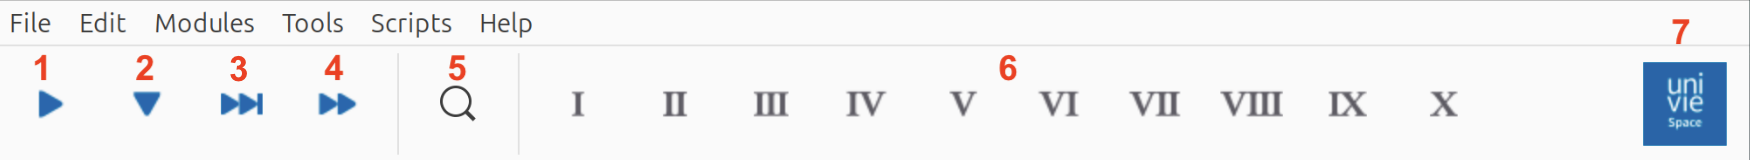
\includegraphics[width=1\linewidth]{Editor_top.png}
    \caption{Top Panel of the Editor}
    \label{editor_top}
\end{figure}

The menu bar at the top of the main window provides access to a range of functions.
While standard items such as \textit{File} and \textit{Edit} behave as expected, a few noteworthy entries specific to \textit{ccs} are highlighted below.\\
\textit{Tools:} Restart the Terminal, for example after switching mibs and reconnecting sql in case of buggy behaviour.\\
\textit{Scripts:} Open and manage frequently used scrips. These can be organized in \texttt{CCS/Ccs/scripts}. 
(In contrast to the action buttons, the file will be opened and -if desired- run by the playback buttons. By pressing an action button, the code will immediately be executed.)

\begin{figure}[h!]
    \centering
    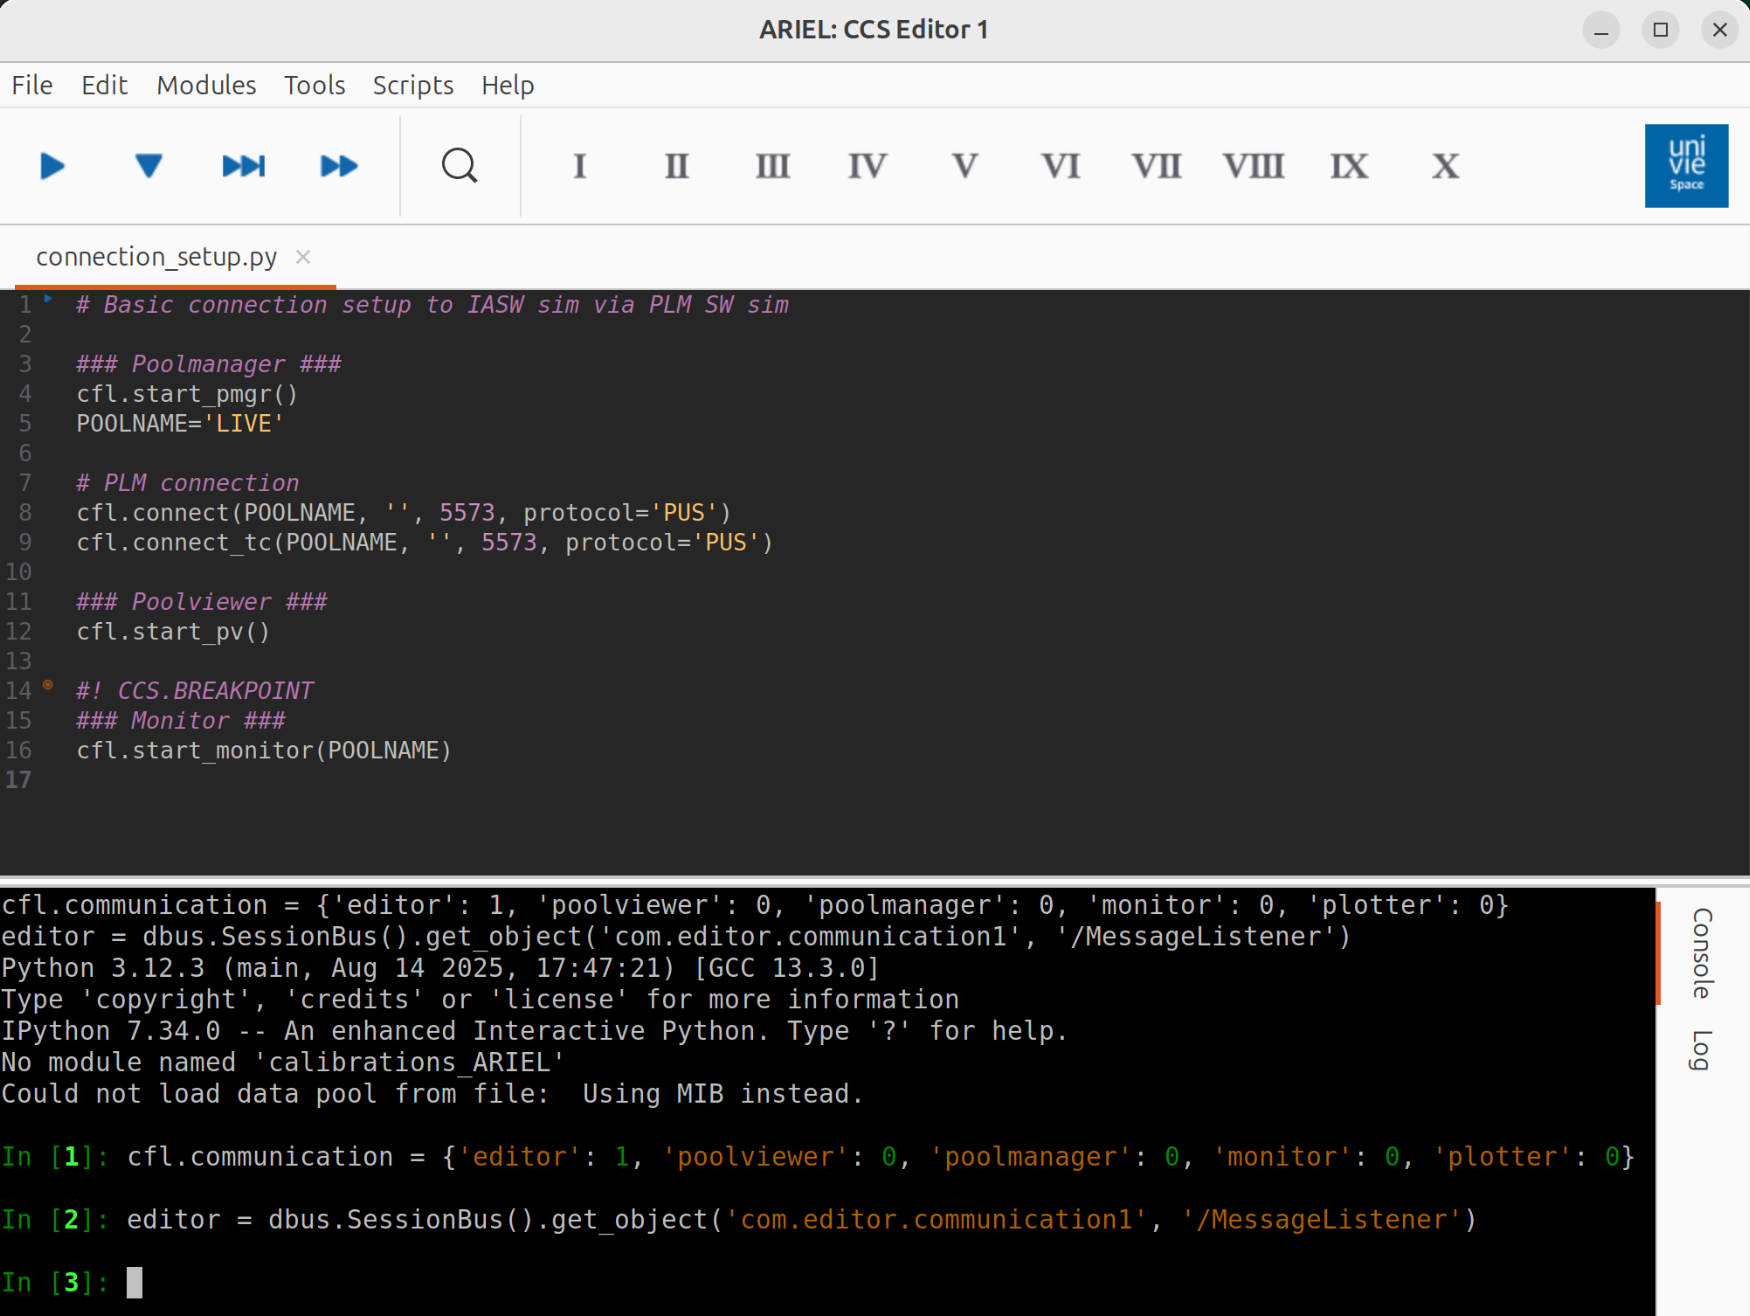
\includegraphics[width=1\linewidth]{Editor_main.png}
    \caption{Welcome screen of \textit{ccs}: the Editor}
    \label{editor}
\end{figure}



%###########################################################################################
\subsection{Pool Manager} \label{manager}
The Pool Manager is responsible for establishing and managing socket connections as well as handling data transfer between CCS and the application. 
When first opened, the window shows nothing in the lower half. Once a connection has been initiated, the active links are listed in the lower part of the interface. \\

The Pool Manager provides a graphical front-end to operations that can also be performed programmatically within the Editor. 
The example below illustrates how the same connections can be created in a script:

\begin{verbatim}
cfl.start_pmgr()
POOLNAME='LIVE'

cfl.connect(POOLNAME, '', 5573, protocol='PUS')
cfl.connect_tc(POOLNAME, '', 5573, protocol='PUS')
\end{verbatim}


\begin{figure}[h!]
    \centering
    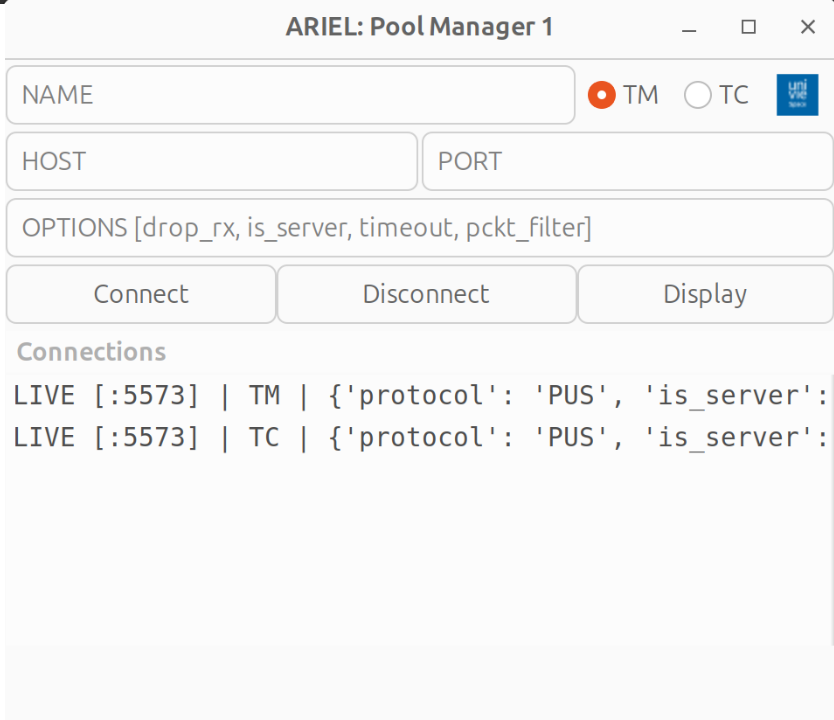
\includegraphics[width=0.4\linewidth]{pool_manager.png}
    \caption{Pool Manager connection according to the parameters set in example script.}
    \label{pool_manager}
\end{figure}

As shown in Figure~\ref{pool_manager}, the GUI provides the same connection options as the \texttt{connection\_setup.py} script. 
When closing the Pool Manager, a prompt appears asking how the process should be terminated. 
Selecting \emph{No} closes only the graphical interface while keeping the Pool Manager running in the background.
To reconnect to the application at a later stage, the Pool Manager must be fully terminated by selecting \emph{Yes}. 
The connection can then be re-established from within the Editor.



\subsection{Pool Viewer}
%quick overview, left and right bif panels
The Pool Viewer provides a live view of the data pool selected in the drop-down menu at the top left of the window (see Figure~\ref{fig:poolviewer} 1). 
It is divided into two main sections:\\

The right panel displays the contents of the pool, with one packet per row. Each entry corresponds to a single TM or TC packet. 
The main header information is shown in the individual columns:

\begin{itemize}
    \item \#: Internal \textit{ccs} counter for received or sent packets, starting at 1
    \item TM/TC: Telemetry or Telecommand
    \item APID: Application Process Identifier
    \item SEQ: Sequence counter (per APID)
    \item len-7: Length in bytes minus 7
    \item ST: Service type
    \item SST: Subservice type
    \item Dest ID: Destination Identifier
    \item Time: Packet timestamp in seconds (relative to application start)
    \item Data: Raw source data in hexadecimal representation
\end{itemize}

The left panel displays the decoded content of the packet currently selected in the list. Parameters, values, and (if applicable) units are shown in structured form.
When clicking on a packet in the right list, the detailed information for that specific TM or TC is displayed in the left panel. 
To return to the live autoscroll mode, where the newest incoming packet is automatically selected, press the \texttt{End} key. 
At the top of the left panel, two checkboxes provide additional options. \textit{Decode Source Data} enables or disables the decoding of packet content. 
If disabled, raw data are displayed in hexadecimal, decimal, and ASCII format. \textit{Calibrated}, when active, textual calibrations (if available) are applied to parameter values. 
For example, the parameter Sid may be shown as \texttt{ESSENTIAL\_HK} instead of its numeric value as can be seen in Figure \ref{fig:poolviewer}. 
By clicking on an individual parameter in the left panel, its raw values are displayed next to the two checkboxes at the top. 
Both the hexadecimal (HEX) and decimal (DEC) representations of the parameter are shown for reference.\\



\begin{figure}
    \centering
    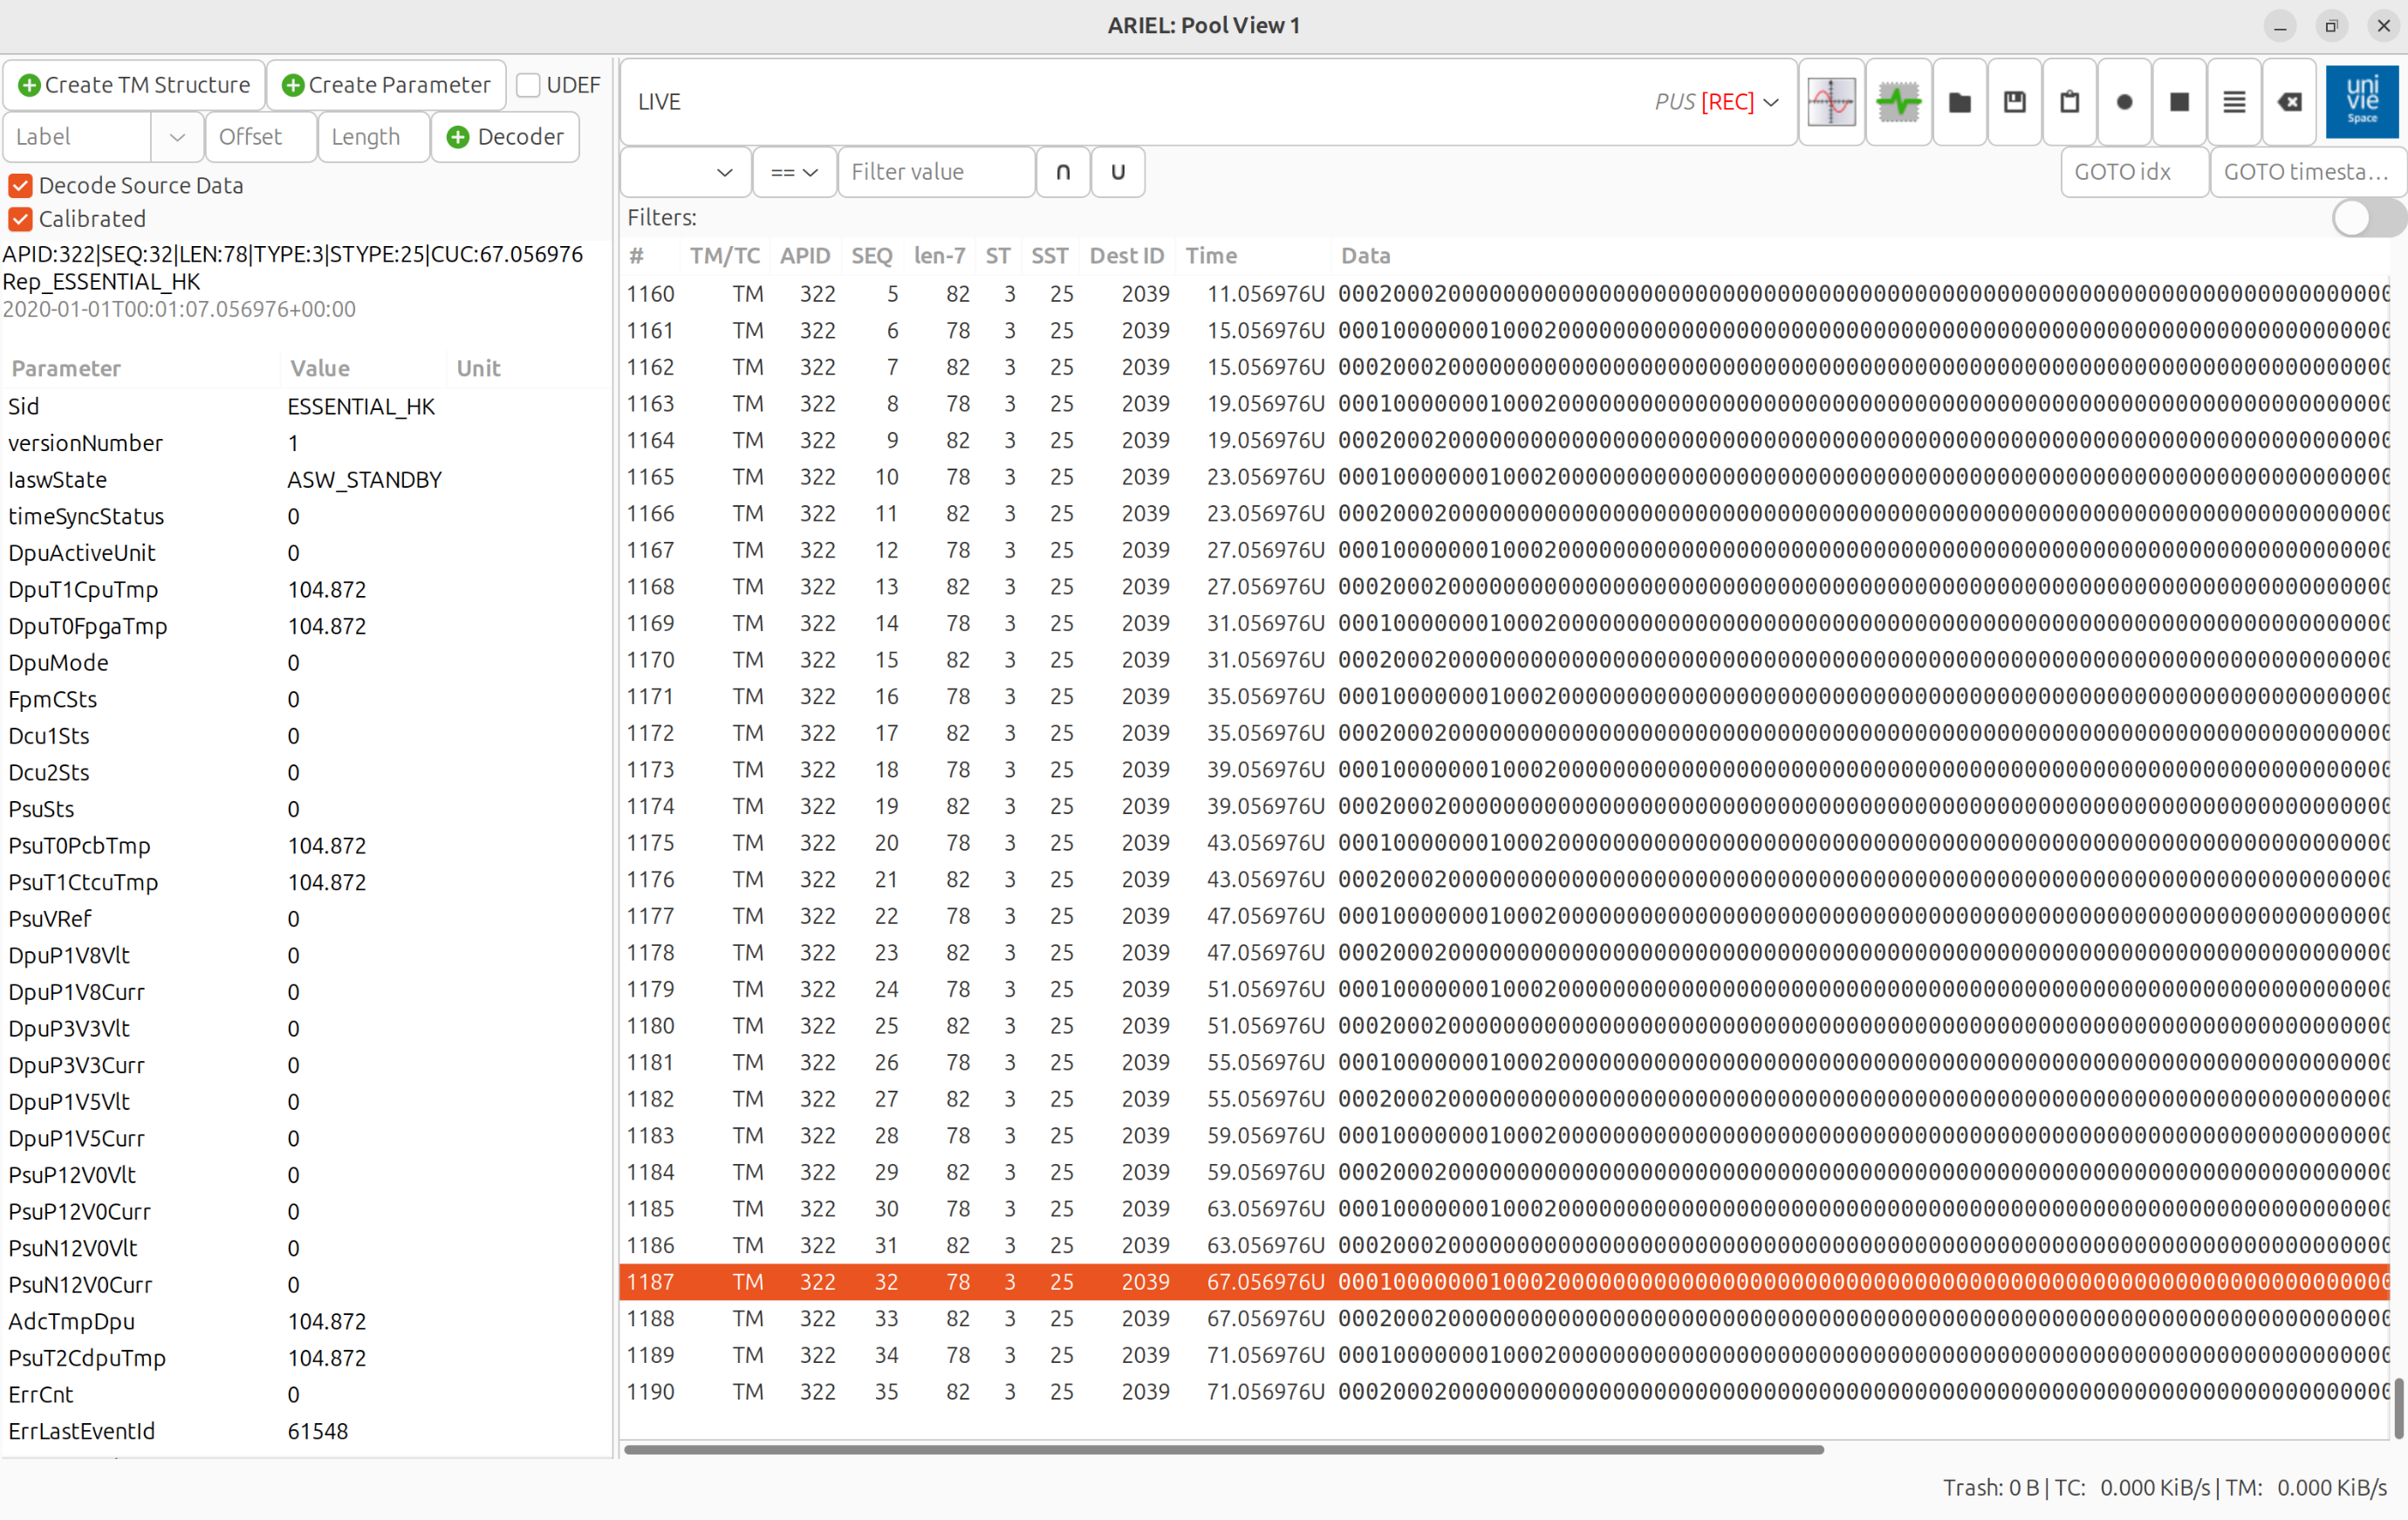
\includegraphics[width=1\linewidth]{PoolViewer.png}
    \caption{Pool Viewer receiving TM(3,25) from Pool "LIVE"}
    \label{fig:poolviewer}
\end{figure}

At the top left of the Pool Viewer, several buttons allow the user to define and modify packet structures:
\begin{itemize}
\item Create TM Structure: Opens a dialog to create a new telemetry packet. The packet can be defined either using parameters already present in the MIB or by combining them with user defined parameters.

\item Create Parameter: Allows the creation of user-defined parameters that can then be included in packet structures or monitored individually.

\item Decoder: Enables the addition of a user-defined decoder to interpret arbitrary bytes within a packet. This provides flexibility in handling data fields not explicitly defined within the MIB.

\item UDEF (User Defined): When the checkbox is enabled, \textit{ccs} prioritizes user-defined packets over those already present in the MIB. For example, if a packet with service/subservice \texttt{(3,25)} is created by the user, and the \emph{UDEF} checkbox is selected, \textit{ccs} will use the user-defined version instead of the MIB entry.

\end{itemize}




\begin{figure}[h!]
    \centering
    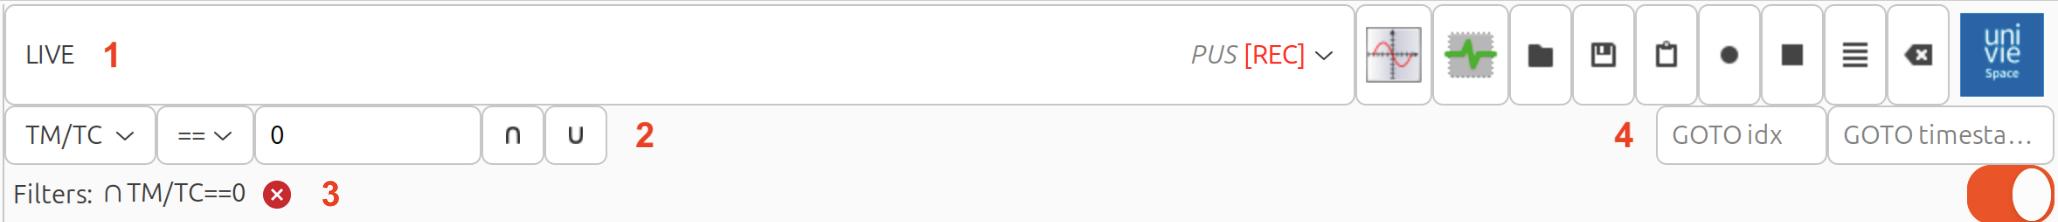
\includegraphics[width=1.1\linewidth]{pool_view_top.png}
    \caption{Top panel pool viewer}
    \label{top_viewer}
\end{figure}

As shown in Figure~\ref{top_viewer}, the controls at the top right of the Pool Viewer are organized into several elements:
\begin{enumerate}
    \item Pool selection (drop-down menu): The drop-down menu determines which pool is currently displayed. Typically, this is the live pool receiving TM packets over the corresponding socket, but it may also be a static pool loaded from disk. Additional pools can be loaded (description below) and selected here.

    \item Filter panel: To ease navigation in large data sets, the filter panel allows the displayed packets to be restricted according to user-defined criteria. Filters can be applied to any of the columns. Multiple conditions can be combined logically, and the toggle button on the right activates or deactivates the filter set. It should be noted that for TM/TC filtering 0 corresponds to TMs and 1 corresponds to TCs.

    \item Active filter display: When a filter is applied, the active conditions are shown below the panel. This provides an overview of which filters are currently in effect.

    \item Navigation fields (GOTO): The two input fields labeled \textit{GOTO} allow direct navigation within the packet list. Users can jump either to a specific index \# or to a packet with a defined timestamp value, avoiding the need to scroll manually through very large pools. It is not necessary to enter the entire timestamp, the first few digits suffice.
\end{enumerate}



\begingroup
\captionsetup[figure]{font=small,labelfont=bf,justification=centering}
\captionsetup[subfigure]{font=small,labelfont=bf,justification=centering,singlelinecheck=false}
\setlength{\abovecaptionskip}{6pt}
\setlength{\belowcaptionskip}{0pt}

\newcommand{\iconheight}{1.1cm}
\newcommand{\iconsubw}{0.18\linewidth}

\newcommand{\iconsvg}[3]{% file(without .svg), caption, label
  \begin{subfigure}[t]{\iconsubw}\centering
    \includesvg[height=\iconheight]{#1}
    \subcaption{#2}\label{#3}
  \end{subfigure}%
}
\newcommand{\iconimg}[3]{% file(with extension), caption, label
  \begin{subfigure}[t]{\iconsubw}\centering
    \includegraphics[height=\iconheight]{#1}
    \subcaption{#2}\label{#3}
  \end{subfigure}%
}

\begin{figure}[ht]
  \centering
  \iconimg{func.png}{Parameter plotter}{fig:icon-plotter}
  \iconimg{monitor.png}{Parameter monitor}{fig:icon-monitor}
  \iconsvg{open}{Open folder / Load pool}{fig:icon-open}
  \iconsvg{save}{Save pool}{fig:icon-save}
  \iconsvg{clear}{Clear current pool}{fig:icon-clear}
  \caption{Icons visible on top of the Pool Viewer. Note that the look of some icons depends on the host environment and can thus vary from system to system.}
  \label{fig:pool-icons}
\end{figure}
\endgroup



In addition to displaying the currently connected TM pool, the viewer can also load packet data stored on disk (e.g., from a previously saved session). 
This is done by selecting the \emph{Load} button \ref{fig:icon-open} in the toolbar and choosing the desired file. 
Once loaded, the data become available through the pool drop-down menu.\\

Conversely, the contents of the active pool can be exported using the \emph{Save pool} button \ref{fig:icon-save}. 
The export may include the entire pool or only selected packets, and can be written in binary, hexadecimal, or decoded CSV format.\\

The \emph{Clear} button \ref{fig:icon-clear} will clear the currently selected pool.
%Caution: This function is irreversible and all data in the respective pool is deleted!\\

In addition to these functions, two further buttons are available in the toolbar: \emph{Parameter Plotter} \ref{fig:icon-plotter} and \emph{Monitor} \ref{fig:icon-monitor}. 
These provide extended analysis and monitoring capabilities. A detailed description of both will be given in the subsequent chapters.










%###########################################################################################
\subsection{Parameter Plotter}

The Parameter Plotter provides a graphical visualization of parameters contained in the currently selected pool (see Figure~\ref{fig:plotter}). 
It allows both live monitoring and offline inspection of parameter trends over time. \\

The right-hand panel lists all parameters available from the active pool or loaded from the MIB. 
Individual parameters can be selected from this list and added to the plot by clicking the \emph{Add} button. 
The \emph{Clear} button removes all plotted parameters.

The \emph{Add User Defined Parameter} button functions identically to the one in the Pool Viewer, enabling users to create custom parameters not defined in the MIB. 
The adjacent buttons allow editing or deleting the selected user-defined parameter. 
In the image, below Service 197, the options \emph{UDEF} - user defined PUS packet - and \emph{User defined} - user defined parameter - can be found.
This is where individual parameters are available.

Activating the \emph{Live Plot} switch enables continuous updating of the display. 
In this mode, new data points are plotted in real time, and the x-axis automatically expands as time progresses.

\begin{figure}
    \centering
    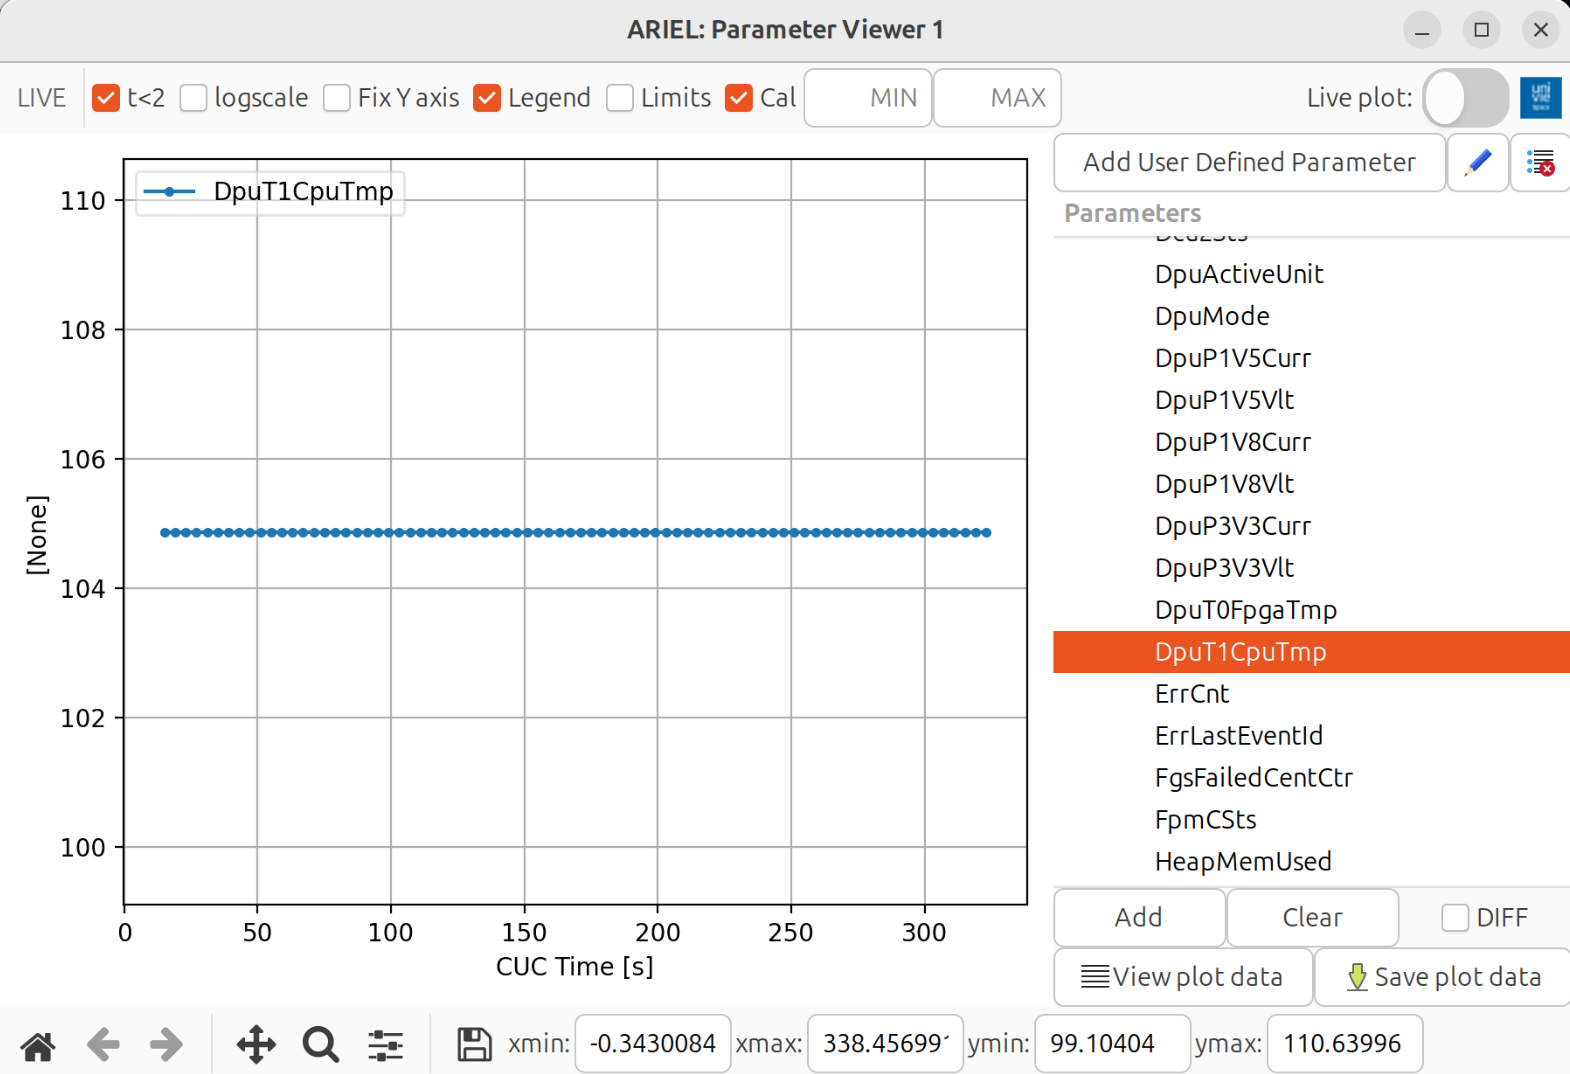
\includegraphics[width=0.7\linewidth]{plotter.png}
    \caption{Parameter Plotter/Viewer: DpuT1CpuTmp parameter displayed in the window.}
    \label{fig:plotter}
\end{figure}

Next to the \emph{Clear} button, the checkbox labeled \emph{DIFF} enables the display of value differences between consecutive time steps for a given parameter.
This allows users to easily track incremental changes rather than absolute values. \\

The buttons \emph{View plot data} and \emph{Save plot data} provide access to the underlying numerical data of the plotted parameters. 
The data are displayed or exported in a structured tabular format. \\

The controls in the lower toolbar correspond to standard Matplotlib navigation functions. 
The \emph{Save plot} button located in this toolbar saves the rendered plot itself—as an image file—rather than its numerical data points.\\

The upper toolbar provides several checkboxes and control buttons that adjust the display and behavior of the plot:

\begin{itemize}

\item t$<$2: Excludes packets with timestamps below two seconds. This avoids displaying data from the initial startup phase, during which the application may not yet be synchronized.

\item logscale: Displays the y-axis on a logarithmic scale.

\item Fix Y axis: Keeps the y-axis range fixed during live updates. This is particularly useful when \emph{Live Plot} is enabled, as it prevents large value jumps from dynamically rescaling the plot.

\item Legend: Toggles the visibility of the parameter legend in the plot area.

\item Limits: Displays parameter limits (if defined in the MIB) as horizontal lines across the plot.

\item Cal: Plots calibrated (engineering) values instead of raw data. The calibration is applied only to the next parameter added.

\item MIN / MAX: Limits the range of packets from which the parameters should be extracted, identified by the pool index (\textbf{\#} column).

\end{itemize}


%###########################################################################################
\subsection{Parameter Monitor} \label{monitor}




The Parameter Monitor module facilitates real-time supervision of selected parameters. 
It can be opened directly from the Pool Viewer via the \emph{Monitor} button (see Figure~\ref{fig:icon-monitor}). \\

The main window displays three counters (\emph{Error LOW}, \emph{Error MEDIUM}, and \emph{Error HIGH}) that indicate the number of parameters currently exceeding their respective soft or hard limits (corresponding to TM(5,2), TM(5,3), TM(5,4)). The \emph{Reset} button clears these alerts, returning the indicators to their default state. 
The \emph{Calibrated} option behaves as in other modules, displaying engineering values when enabled.\\

New parameter sets can be configured via the \emph{Set Parameters} button, which opens the \emph{Monitoring Setup} dialog (Figure~\ref{fig:monitorsetup}). 
Within this window, parameters can be added or removed and grouped into predefined sets. 
Each configuration can be assigned a label for later retrieval, or an existing configuration can be reloaded from disk. \\

\begin{figure}
    \centering
    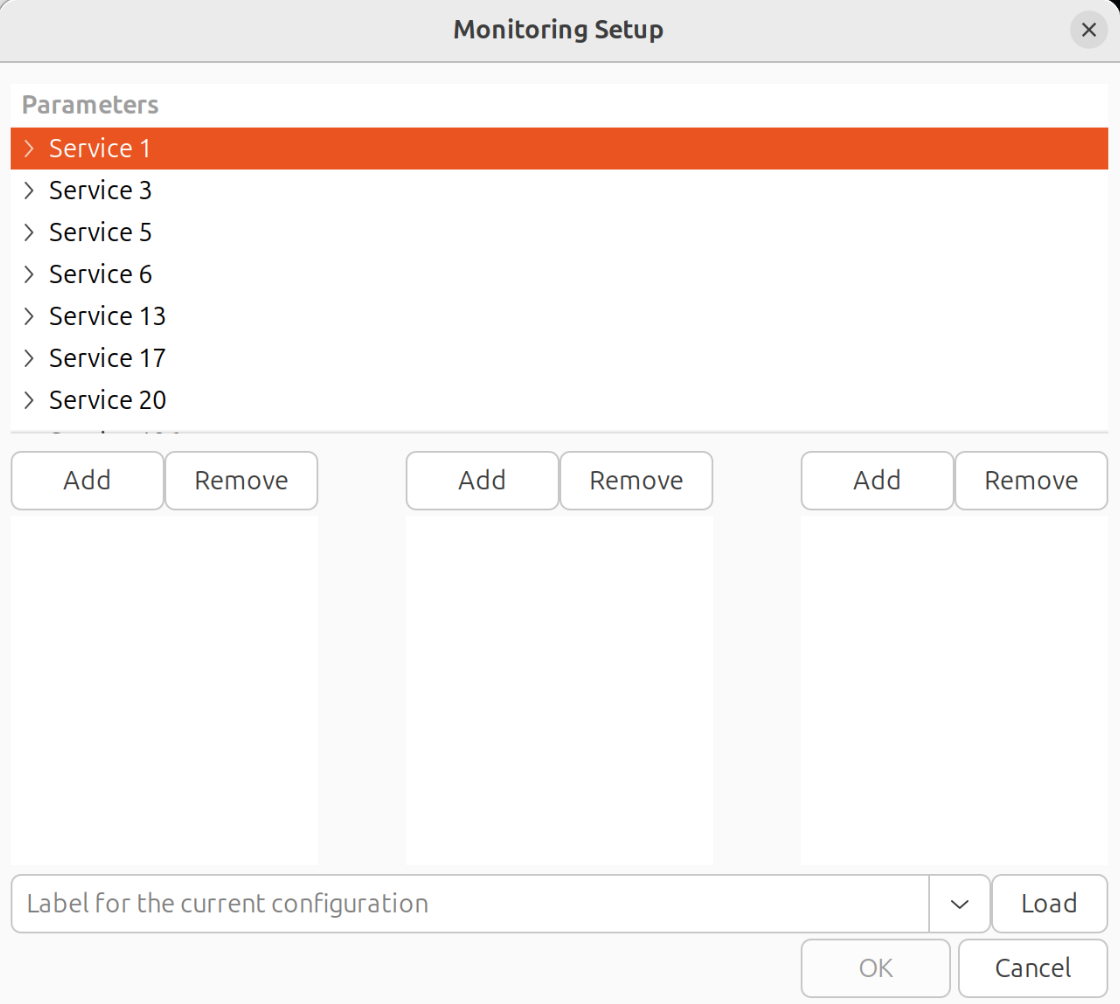
\includegraphics[width=0.6\linewidth]{monitor_setup.png}
    \caption{Parameter Monitor Setup for Parameter selection}
    \label{fig:monitorsetup}
\end{figure}

For each monitored parameter, range checks are performed periodically. If defined in the MIB, both soft and hard limits are applied automatically. 
Parameters are color-coded according to their current status:

\begin{itemize}
\item Green: Value within nominal range
\item Orange: Soft limit exceeded
\item Red: Hard limit exceeded
\item Grey: Parameter not updated within the specified timeout period (the timeout duration is configurable in the config file)
\end{itemize}

\begin{figure}
    \centering
    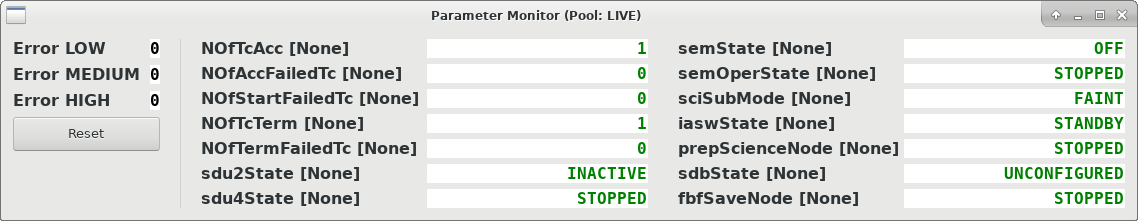
\includegraphics[width=1\linewidth]{monitor_0.png}
    \caption{Parameter Monitor}
    \label{fig:monitor0}
\end{figure}

Hovering the cursor over a parameter displays its defined hard and soft limits will be displayed in a tooltip.



%###########################################################################################
\chapter{Configuration Editor}
\label{config}
The Configuration Editor provides a graphical interface for viewing and modifying the various configuration files (.cfg) used by \textit{ccs}.
It serves a similar purpose to a preferences window, allowing the user to inspect and adjust system parameters without manually editing configuration files. 
It can be launched in two ways:

\begin{itemize}
    \item From the terminal: navigate to the \texttt{CCS} directory and run \texttt{./start\_config\_editor}
    
    \item From within the \textit{ccs} editor: via the top menu bar under Edit and Preferences
\end{itemize}

Upon opening, multiple configuration files are displayed as tabs. Each tab corresponds to one configuration file and lists its editable entries organized by section. 
Changes are applied automatically when the application, to which the change has been applied, is restarted. 
The most relevant files are \texttt{egse.cfg}, which is responsible for general configuration of database and project information for the setup process and \texttt{ccs\_main\_config.cfg} for editor style preferences.

\begin{figure}
    \centering
    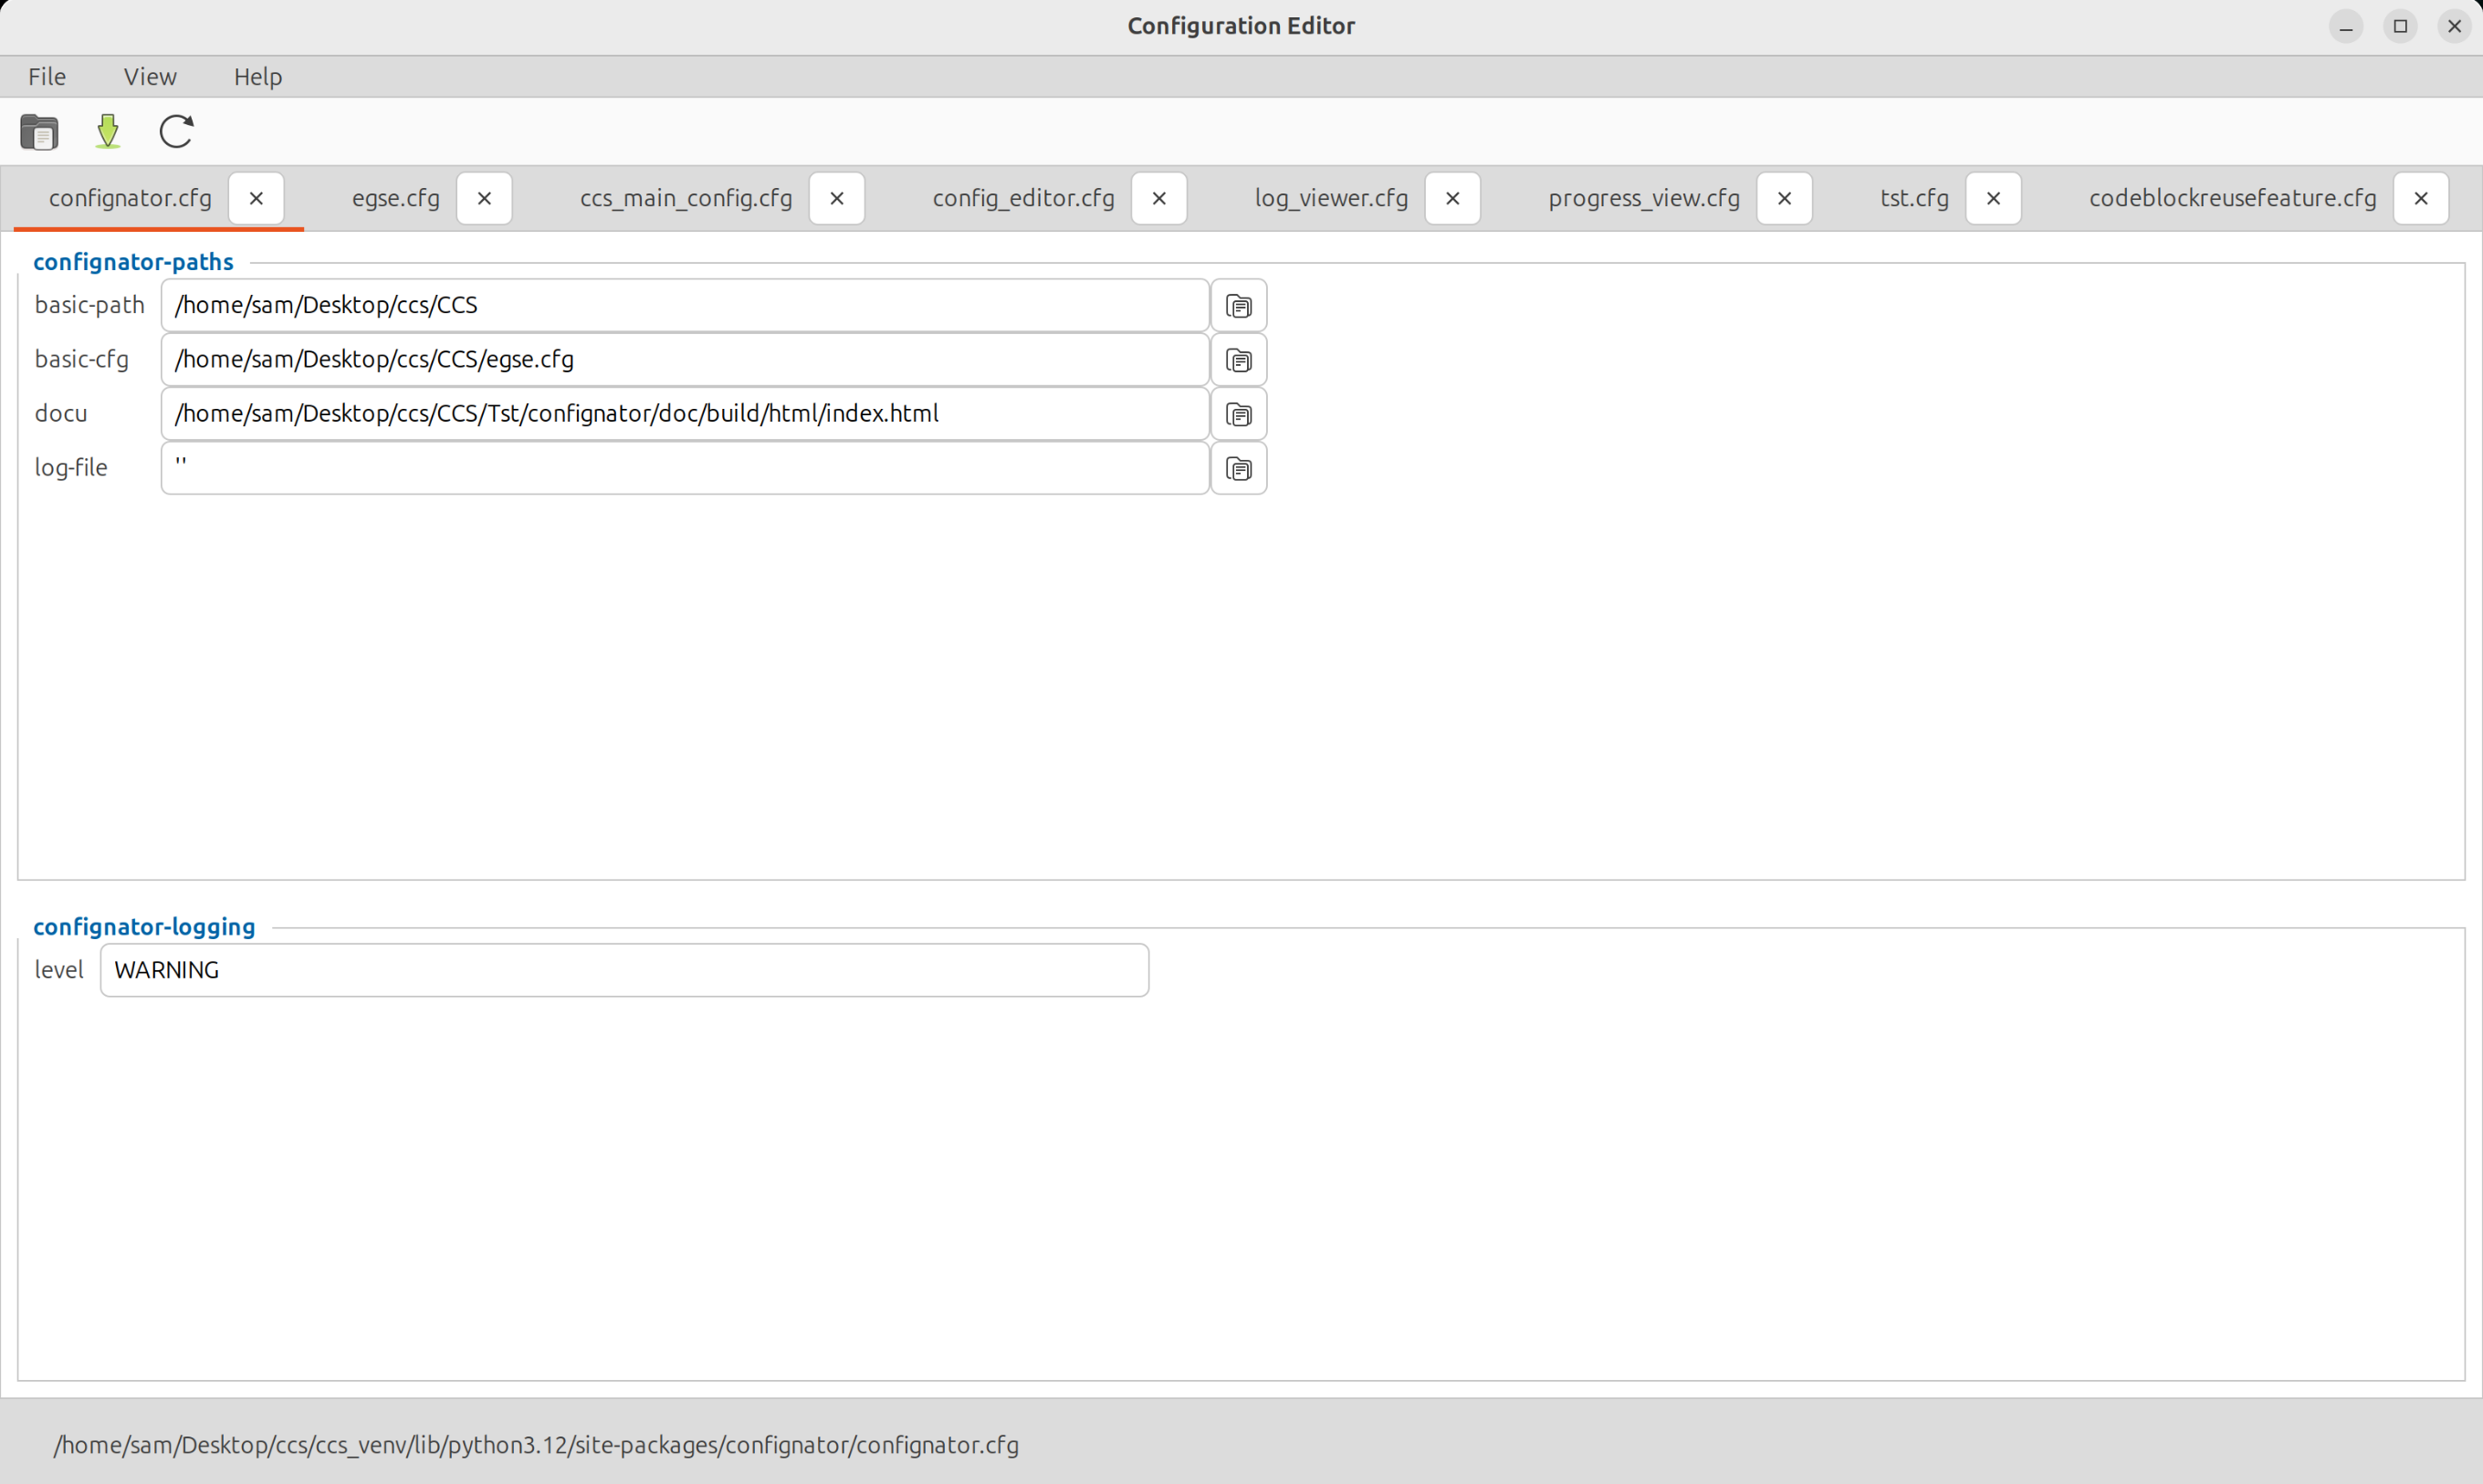
\includegraphics[width=1\linewidth]{config_edit.png}
    \caption{Welcome screen of the Configuration Editor}
    \label{fig:confi_edit}
\end{figure}
While most entries in the \texttt{ccs\_main\_conifg.cfg} file are self-explanatory, a few parameters are worth highlighting due to their relevance for daily \textit{ccs} operation:

\begin{itemize}
    \item ccs-logging: The logging level determines the verbosity of console and log output. Options include DEBUG, INFO, WARNING, and ERROR

    \item ccs-viewer: The parameter drag\_report\_fmt controls the format used when dragging telemetry data from the Pool Viewer to other tools

    \item ccs-monitor: Configuration of the Parameter Monitor module (see Section \ref{monitor}):

    \begin{itemize}
    \renewcommand\labelitemi{--} 
    \item interval: internal refresh rate of the monitor in seconds
  
    \item max\_age: time threshold (in seconds) after which a parameter is considered outdated and is displayed grey
    \end{itemize}

    \item ccs-actions: Entries listed here correspond to the customizable action buttons in the \textit{ccs} editor toolbar (see Figure \ref{editor_top}), script paths as well as the associated icons can be edited (paths are given relative to the directory \texttt{/CCS/Ccs/scripts/})

    \item ccs-pool\_colour\_filters: display colors for TM and TC packets within the pool viewer (filter rule associates color with given service and subtype) or for example in the editor type: pv.add\_colour\_filter({'APID': 322, 'colour' : 'blue'}) for all packets with APID 322 to be displayed in blue
    
\end{itemize}

Note(ccs-monitor\_parameter\_sets): parameter sets defined in the parameter monitor can only be deleted or renamed manually within the configuration file — the GUI does not support removal or renaming of entries.



%###########################################################################################
\chapter{Test Specification Tool}

\begin{figure}
    \centering
    
\includegraphics[width=0.9\linewidth]{tst.png}
    \caption{Test Specification Tool welcome screen}
    \label{fig:tst}
\end{figure}

The Test Specification Tool (tst) is used to define, organize, and execute automated or semi-automated tests for the \textit{ccs} application. 
It provides an integrated interface for creating test sequences, specifying pre- and post-conditions, adding comments, and managing structured test steps. 
Each test can be stored in JSON. \\

Within the tst interface (see Figure~\ref{fig:tst}), users can define test cases by combining command sequences, initialization code, and validation steps. 
When a test step is executed - such as sending a specific telecommand (e.g., \texttt{TC(17,1)}) - the corresponding action is performed directly through \textit{ccs}. 
The response and resulting telemetry can then be observed in real time within the Pool Viewer. The tool therefore acts as a bridge between test definition and system verification.

\section{Getting started}
The Test Specification Tool can be launched in two ways. When working in a terminal within the main \texttt{CCS} directory, the application can be started by executing
\texttt{./start\_tst}. Alternatively, if \textit{ccs} or any of its modules are already running, tst can be opened directly via the menu bar by selecting the corresponding entry. \\

Conversely, \textit{ccs} can also be launched from within the tst interface. The functions of the associated toolbar buttons will be described in detail in the following sections.



%###########################################################################################
\section{Functionality/Interface}
The right section of the Test Specification Tool provides access to several reference tables and views derived from the currently loaded MIB and test files (see Figure~\ref{fig:tst_mib}). This panel serves as a convenient lookup and selection area for telecommands, telemetry packets, and related data structures.

The available tabs at the top include:

\begin{itemize}
\item Code Snippets: Library of reusable test steps. Add a snippet: drag the header of an existing step in the test sequence into the Code Snippets panel. The selected step - including its description, command code, verification logic, and comments - will be stored as a reusable snippet. Reuse the snippet: drag the desired line into the wanted position in the step sequence.
\item TC Table: Displays all telecommands defined in the loaded MIB, including type, subtype, short name, and description.
\item TM Table: Lists the telemetry packets corresponding to the selected MIB including type, subtype, APID, PI1value and description.
\item Data Pool: Provides access to the currently active data pool variables. By right clicking on a row, PID, Name and Name as a string can be copied.
\item Verification: Access to verification routines that can be used to validate the outcome of executed test steps. Drag the desired verification entry from the list into the \emph{Verification Code} section of a test step. The corresponding code will be inserted automatically.
\item Log View: Of the test tool itself, no log information concerning executed tests.
\item JSON View: Displays the JSON structure of the currently loaded or edited test specification file.
\end{itemize}

Right below these tabs - depending which one is currently opened - an option for filtering the content is provided. When a telecommand or telemetry packet is selected, the corresponding parameters are displayed in the lower part of the panel. Each row represents a parameter contained in the selected packet:

\begin{itemize}
\item POS: Position of the parameter within the packet.
\item Parameter: Name of the parameter as defined in the MIB.
\item Datatype: Data type of the parameter.
\end{itemize}

Selecting a parameter row reveals additional information—if available—in the bottom-right corner of the panel. Here, the following details are displayed:

\begin{itemize}
\item Min / Max: Numerical boundaries or enumeration range.
\item Text: Text calibration or descriptive label corresponding to the parameter value.
\item Val: Current or assigned enumeration value.
\end{itemize}

\begin{figure}
    \centering
    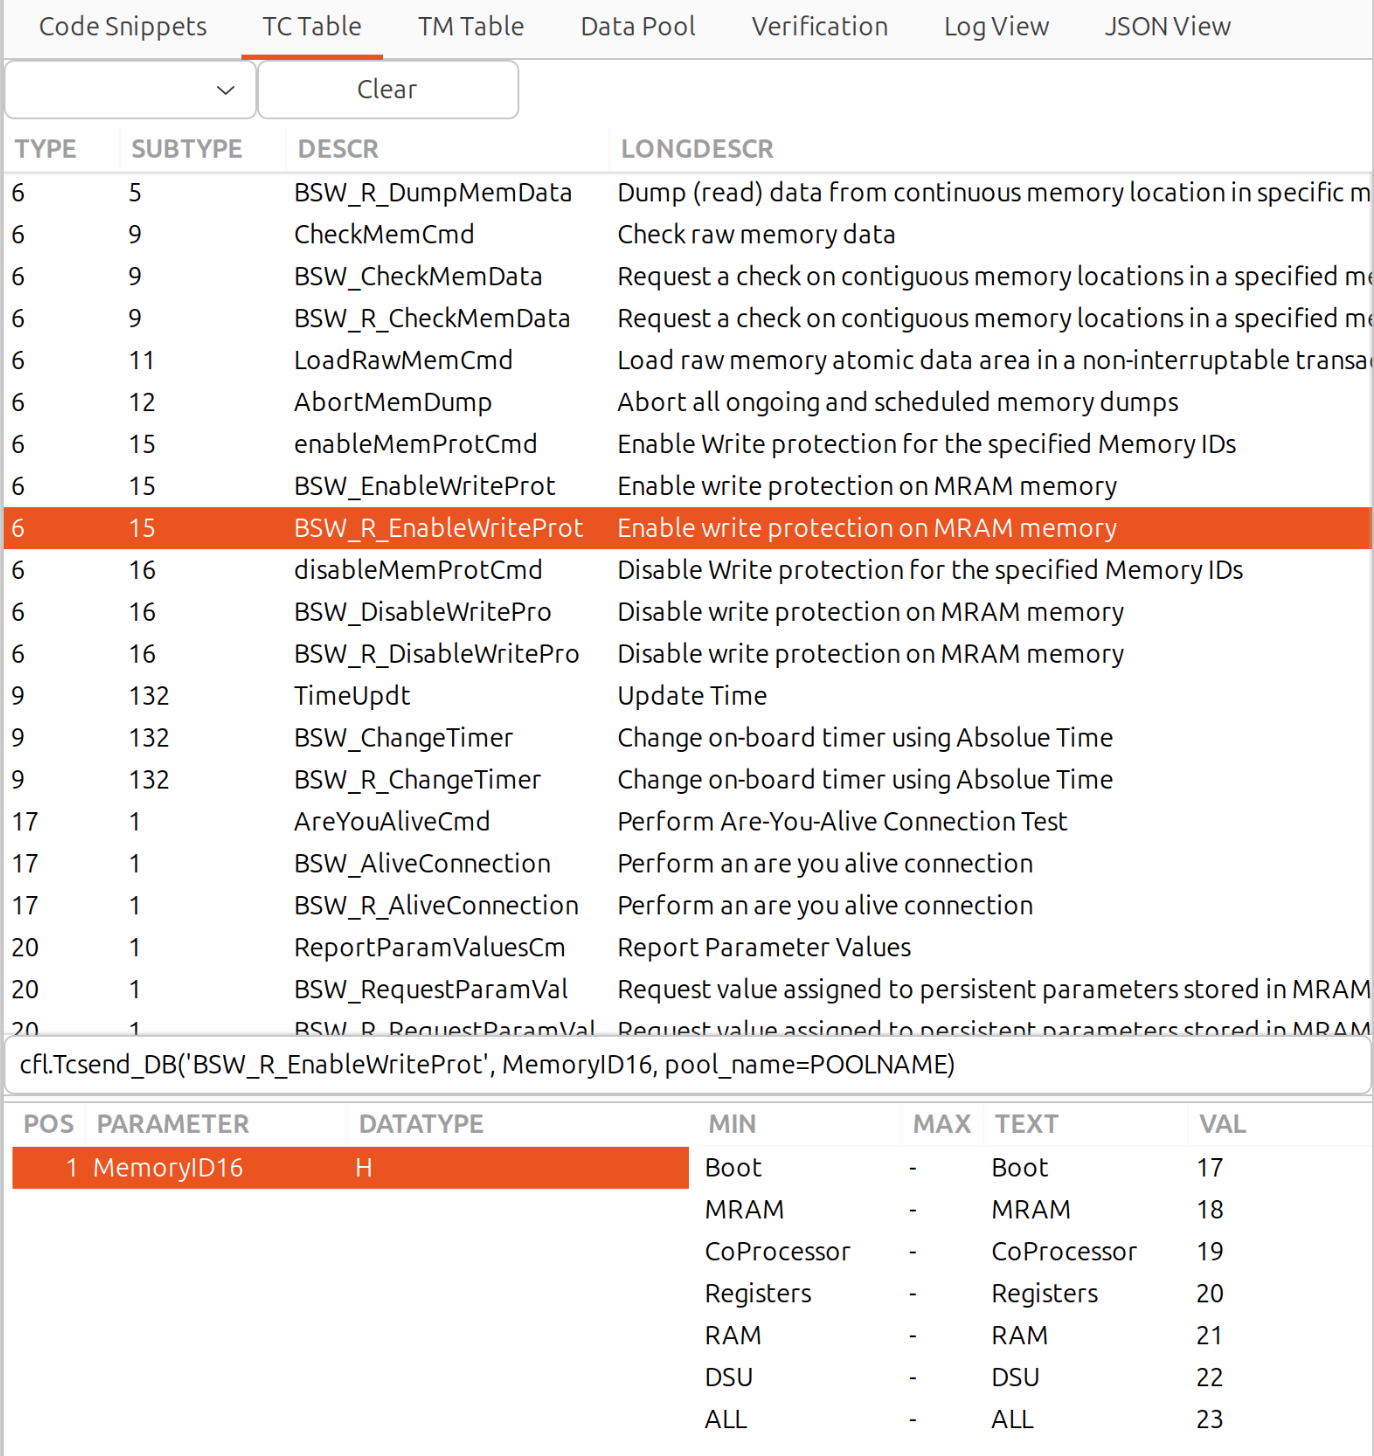
\includegraphics[width=0.8\linewidth]{tst_right.png}
    \caption{Table view of the mib}
    \label{fig:tst_mib}
\end{figure}

Telecommands or telemetry listed in the right-hand panel can be inserted directly into the test definition or into the \textit{ccs} editor via drag and drop. 
This feature automatically generates the corresponding Python command template based on the selected MIB entry. 
For example, dragging the command \texttt{TC(3,3) DelHkCmd} from the \emph{TC Table} into a text editor produces the following code snippet:


\begin{verbatim}
# TC(3,3)DelHkCmd [JA0C0010]
# Delete a Housekeeping or Diagnostic Parameter Report Structure
NParam = None  # JA0H0198
SidNoCal = None  # JA0H0533
cfl.Tcsend_DB('DelHkCmd', NParam, SidNoCal, pool_name=POOLNAME)
\end{verbatim}


\begin{figure}
    \centering
    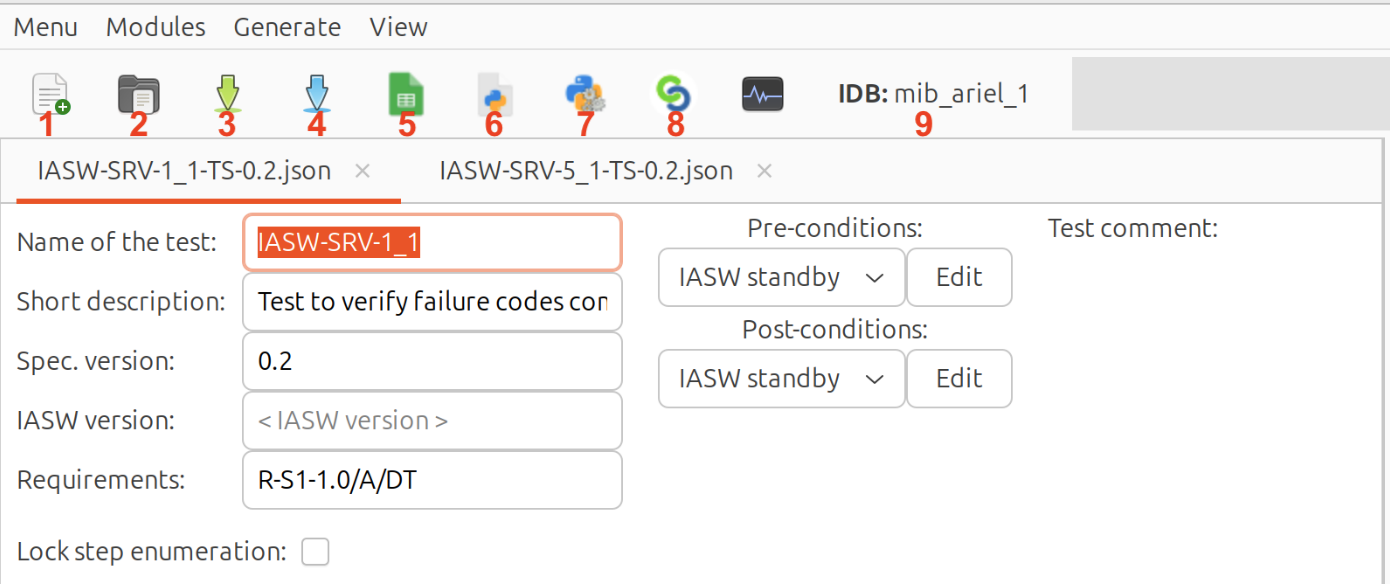
\includegraphics[width=0.5\linewidth]{tst_left_top.png}
    \caption{Overview of tst functions}
    \label{fig:tst_left_top}
\end{figure}

The upper toolbar and menu bar of the Test Specification Tool (see Figure~\ref{fig:tst_left_top}) provide quick access to the most common file and generation functions. 
The options \emph{Menu}, \emph{Modules}, and \emph{View} contain standard options. The \emph{Generate} menu includes the same functions as buttons~5–7 in the toolbar:
\begin{itemize}
\item Generate scripts – corresponds to button~7
\item Export to compact script – corresponds to button~6
\item Export to CSV – corresponds to button~5
\end{itemize}

The numbered toolbar icons are assigned as follows:
\begin{itemize}
\item[1.] Create a new test specification
\item[2.] Open an existing specification file
\item[3.] Save the current specification
\item[4.] Save the current specification under a new name (\emph{Save As})
\item[5.] Export the current test specification as a CSV file
\item[6.] Generate a compact Python script for the current test
\item[7.] Generate a set of Python scripts for automated testing
\item[8.] Launch the \textit{ccs} Editor
\item[9.] Select the active MIB
\end{itemize}

Buttons~6 and~7 both generate executable Python scripts but differ in functionality and workflow. 
Automated Script: Creates four separate files—a command file, a verification file, a run file, and a preparation file. 
The preparation script can be executed beforehand, while the run file sequentially executes the command and verification scripts. 
This method is not generally recommended, as the generated files may be overwritten.
Compact Script: Generates a complete and organized Python script, which can be saved under a custom name and location. 
When the optional \emph{Reporting} checkbox is enabled, a dialogue appears for entering test comments and metadata while executing the test. 
The reporting workflow is described in detail in Section~\ref{sec:exectest}. \\

The upper section of the main window contains the general metadata fields for each test specification, such as the \emph{Name of the test}, \emph{Short description}, \emph{Specification version}, \emph{IASW version}, and associated \emph{Requirements}. 
These fields serve primarily for documentation purposes. \\

The \emph{Pre-conditions} and \emph{Post-conditions} define the expected system states before and after the execution of a test. 
Each can be selected from a drop-down menu. By clicking the \emph{Edit} button next to either field, existing conditions can be modified or new ones created. \\

If the \emph{Lock step enumeration} checkbox is activated, step numbering remains fixed even when additional steps are inserted. 
New steps inserted between existing ones are automatically assigned a sub-index (e.g., inserting a step between steps 2 and 3 will result in step 2.1). \\


\begin{figure}
    \centering
    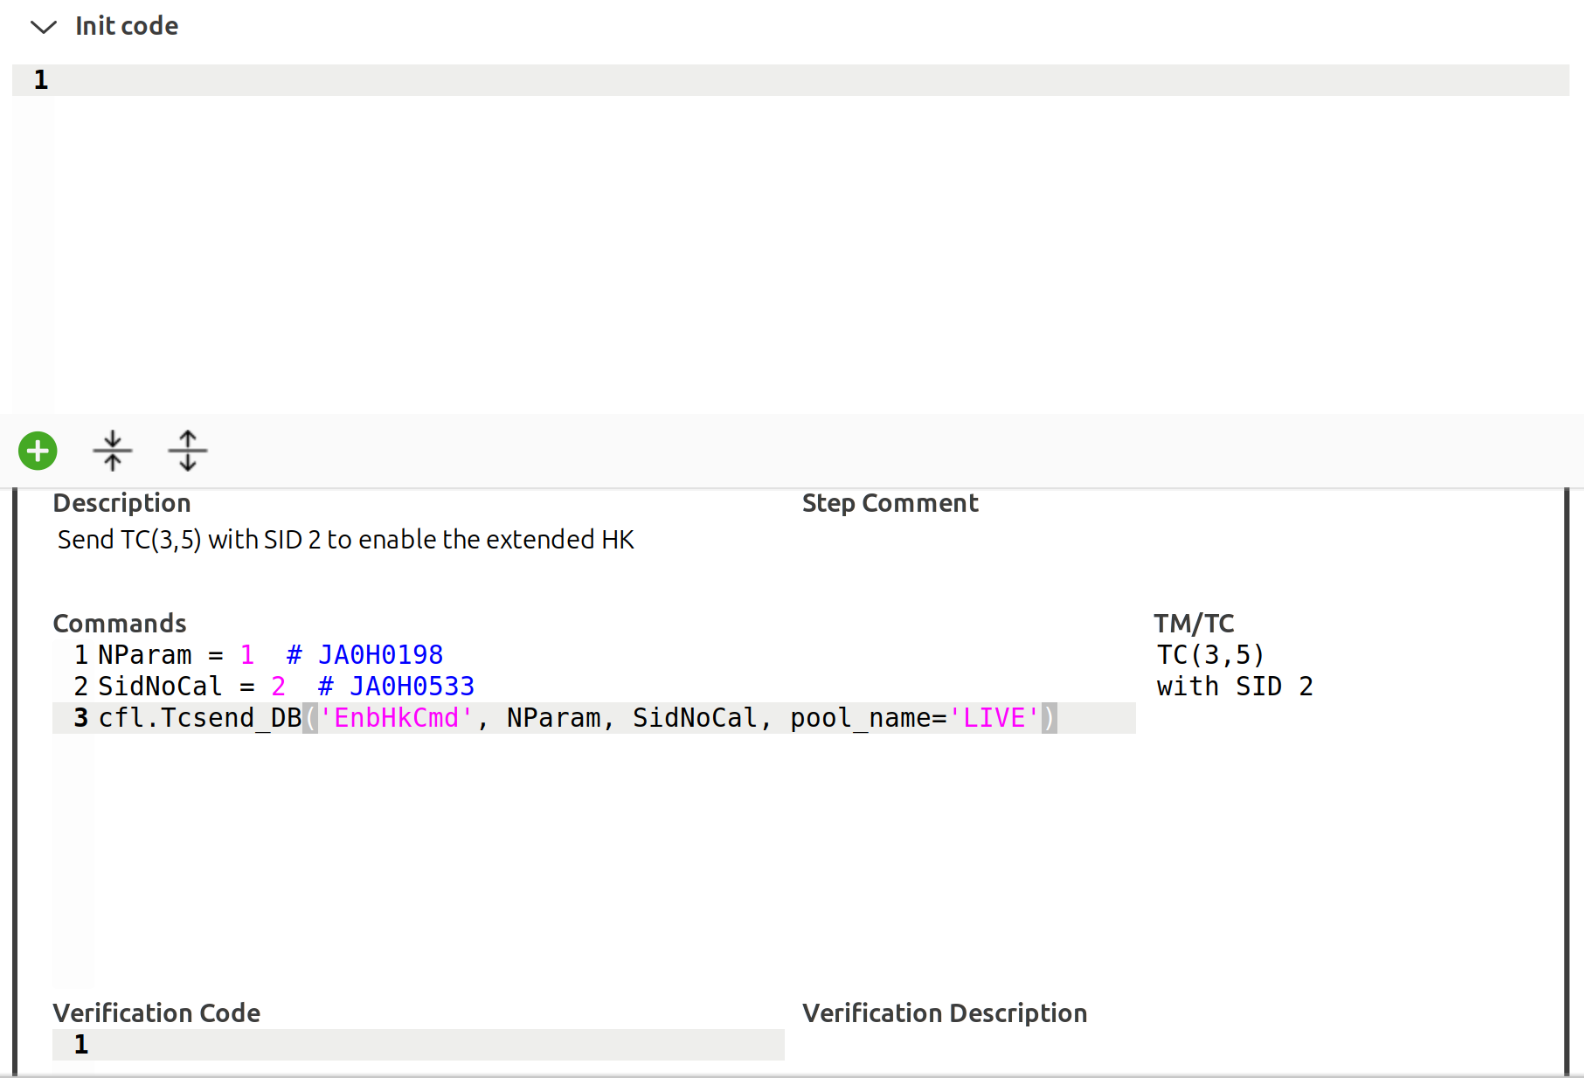
\includegraphics[width=0.5\linewidth]{tst_left_open.png}
    \caption{Singular test step of command TC(3,2)}
    \label{fig:tst_left_open}
\end{figure}

\begin{figure}
    \centering
    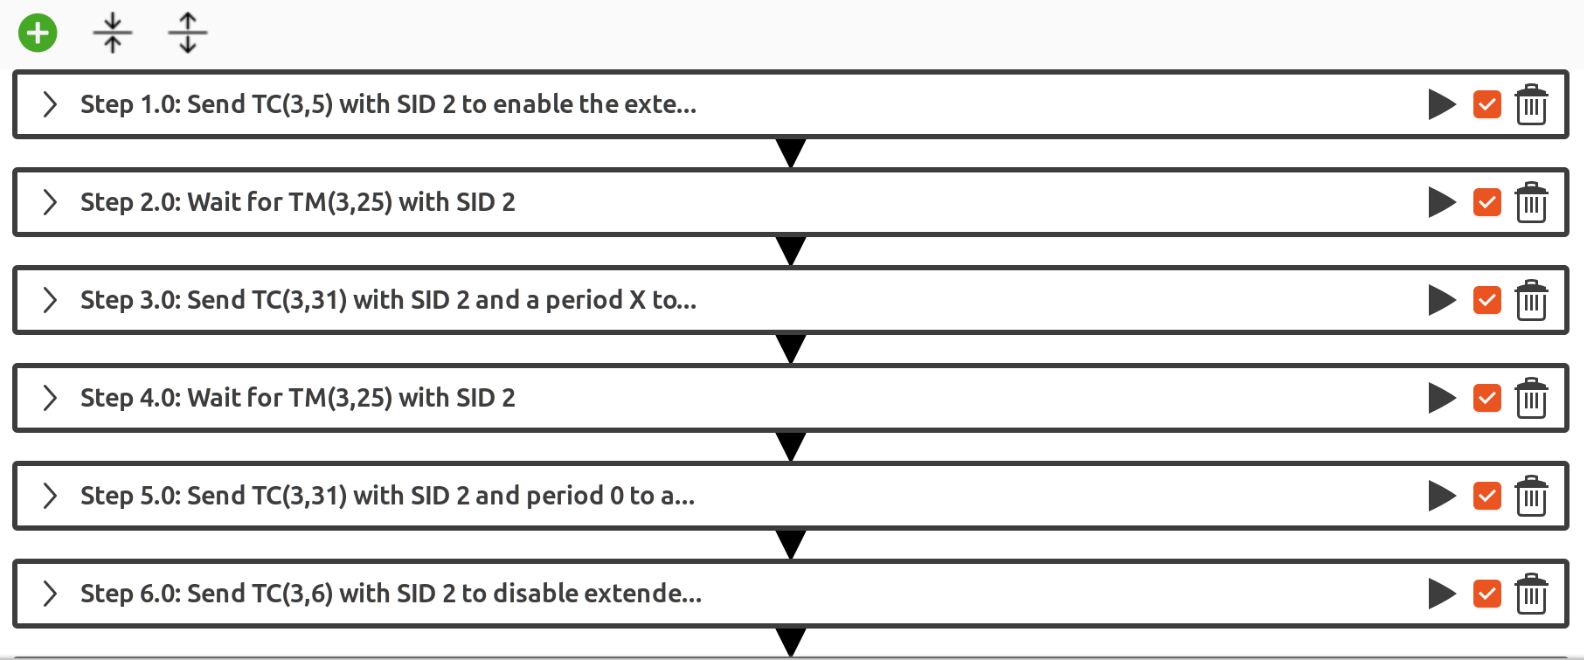
\includegraphics[width=0.5\linewidth]{tst_left_steps.png}
    \caption{Overview os the test steps in the opened file}
    \label{fig:tst_left_steps}
\end{figure}

Figure \ref{fig:tst_left_steps} displays the test steps of a loaded test specification for service 3. 
Above the test step in Figure \ref{fig:tst_left_open}, an \emph{Init code} field is provided. 
Code entered here is executed once before any of the test steps and remains valid throughout the entire test. 
It can be used, for example, to define variables or perform initial setup actions required for subsequent commands. \\

Below the initialization section, the test steps are displayed in sequential order. 
In order to view the details of an individual step, simply click on the desired step and something similar to Figure \ref{fig:tst_left_open} will be displayed. 
The toolbar buttons above the list of steps provide following functionalities:
\begin{itemize}
\item Plus: Adds a new step at the end of the list
\item Middle button: Collapses all expanded steps
\item Right button: Expands all steps to show their detailed contents
\end{itemize}


Individual steps can also be rearranged by drag and drop, the numbering is automatically updated to maintain a consistent sequence. 
To insert a new step between existing ones, right-click in the empty space between two steps and choose either \emph{Insert step above} or \emph{Insert step below}.

Each step includes three control buttons on its right-hand side:
\begin{itemize}
\item Play: Executes only the selected step
\item Checkbox: Toggles whether the step is active
\item Trash: Deletes the step from the sequence
\end{itemize}


When a test step is expanded, several editable fields are displayed that define its content and behavior. 
The \emph{Description} field specifies the purpose of the step and is also shown next to the step number in the main list. \\

The \emph{Command} section contains the actual code to be executed. 
Commands can either be written manually or inserted by dragging a telecommand (e.g., \texttt{TC(3,5)}) from the right-hand panel. 
Parameters such as \texttt{SID} or other command arguments can then be filled in as required.\\

The \emph{Step Comment} field can be used to provide additional notes or explanations relevant to the current step.\\

The \emph{TM/TC Comment} indicates which telemetry or telecommand is involved in the step—for example, \texttt{TC(3,5) with SID 2}.\\

The \emph{Verification Code} field allows inserting verification routines, either written directly or added via drag and drop from the \emph{Verification} panel on the right-hand side. 
The accompanying \emph{Verification Description} provides a brief textual summary of the expected verification behavior.\\




%###########################################################################################
\section{Executing a test}
\label{sec:exectest}
Before using the Test Specification Tool and performing drag-and-drop operations involving telemetry packets during test verification, one configuration parameter in the \textit{ccs} setup must be checked.

\begin{enumerate}
    \item In the \textit{ccs} editor, open the preferences dialog from the edit menu
    
    \item In the configuration editor, select the file \emph{ccs\_main\_config.cfg} from the tab bar

    \item Locate the section \emph{ccs-viewer} and find the entry \emph{drag\_report\_fmt}

    \item Ensure that the value is set to 2
    
\end{enumerate}


This parameter defines how telemetry data are formatted when dragged from the Pool Viewer into other tools:
\begin{itemize}
    \item 0: Paste data as raw byte strings
    \item 1: Paste data in tex table format
    \item 2: Paste data in structured format recognized by the test verification dialog
\end{itemize}
If this value is not set to 2, telemetry packets dragged during test verification will not be recognized correctly in the verification window.\\

The following example illustrates the complete workflow of defining and executing a simple test case using the Test Specification Tool and the \textit{ccs} Editor. 
The test verifies that the connection to the application is functional by sending the telecommand \texttt{TC(17,1)} and checking for the corresponding telemetry response \texttt{TM(17,2)}. \\

Creating the test specification:
\begin{enumerate}
    \item Start the Test Specification Tool
    
    \item Open a new file and load the corresponding MIB using the selector in the top right corner
    
    \item Enter the general test information such as the Name, Short Description, Specification Version, and Requirement Reference
    
    \item Enter a suitable Description for the first step, e.g.
    \emph{“Send TC(17,1) to verify that the connection to the IASW is working.”} (The rest of the fields will be left empty in this example for simplicity)
    
    \item In the right-hand panel, navigate to the TC Table, locate the command \texttt{TC(17,1)}, and drag it into the \emph{Command} field of the step
    
    \item Create a second step by clicking the “+” button
    
    \item Expand the step and enter a description, for example
    \emph{“Wait for TM(17,2)”}
\end{enumerate}


Once all steps are defined, open the Generate menu and select
\emph{“Export to compact script”}. Choose a save location and enable the Reporting option in the bottom-right corner of the export dialog. 
Confirm to generate the test files. \\

After the test file is generated, open the \textit{ccs} editor and ensure that the application is connected and running - execute the \texttt{connection\_setup.py} script to establish communication. 
From the menu, open the generated test file (e.g., \texttt{SRV-17\_1\_TS-0.1.py}). 
This script can now be run from within the editor. Mind the fact that there are several breakpoints in the script. 
The code from the example above is shown in Figure \ref{fig:test_editor}. 
Upon execution, a series of GUI dialogues will appear guiding the user through the test process.
The conditions for the test will be visible in the console of the editor as comments. \\

The first dialogue requests confirmation to execute the current step (see Figure~\ref{fig:dialog_1}). 
When confirmed, the corresponding telecommand \texttt{TC(17,1)} is sent, and the telemetry response \texttt{TM(17,2)}—along with related verification telemetry from Service 1—can be observed in the Pool Viewer (Figure~\ref{fig:test_viewer}). \\


\begin{figure}
    \centering
    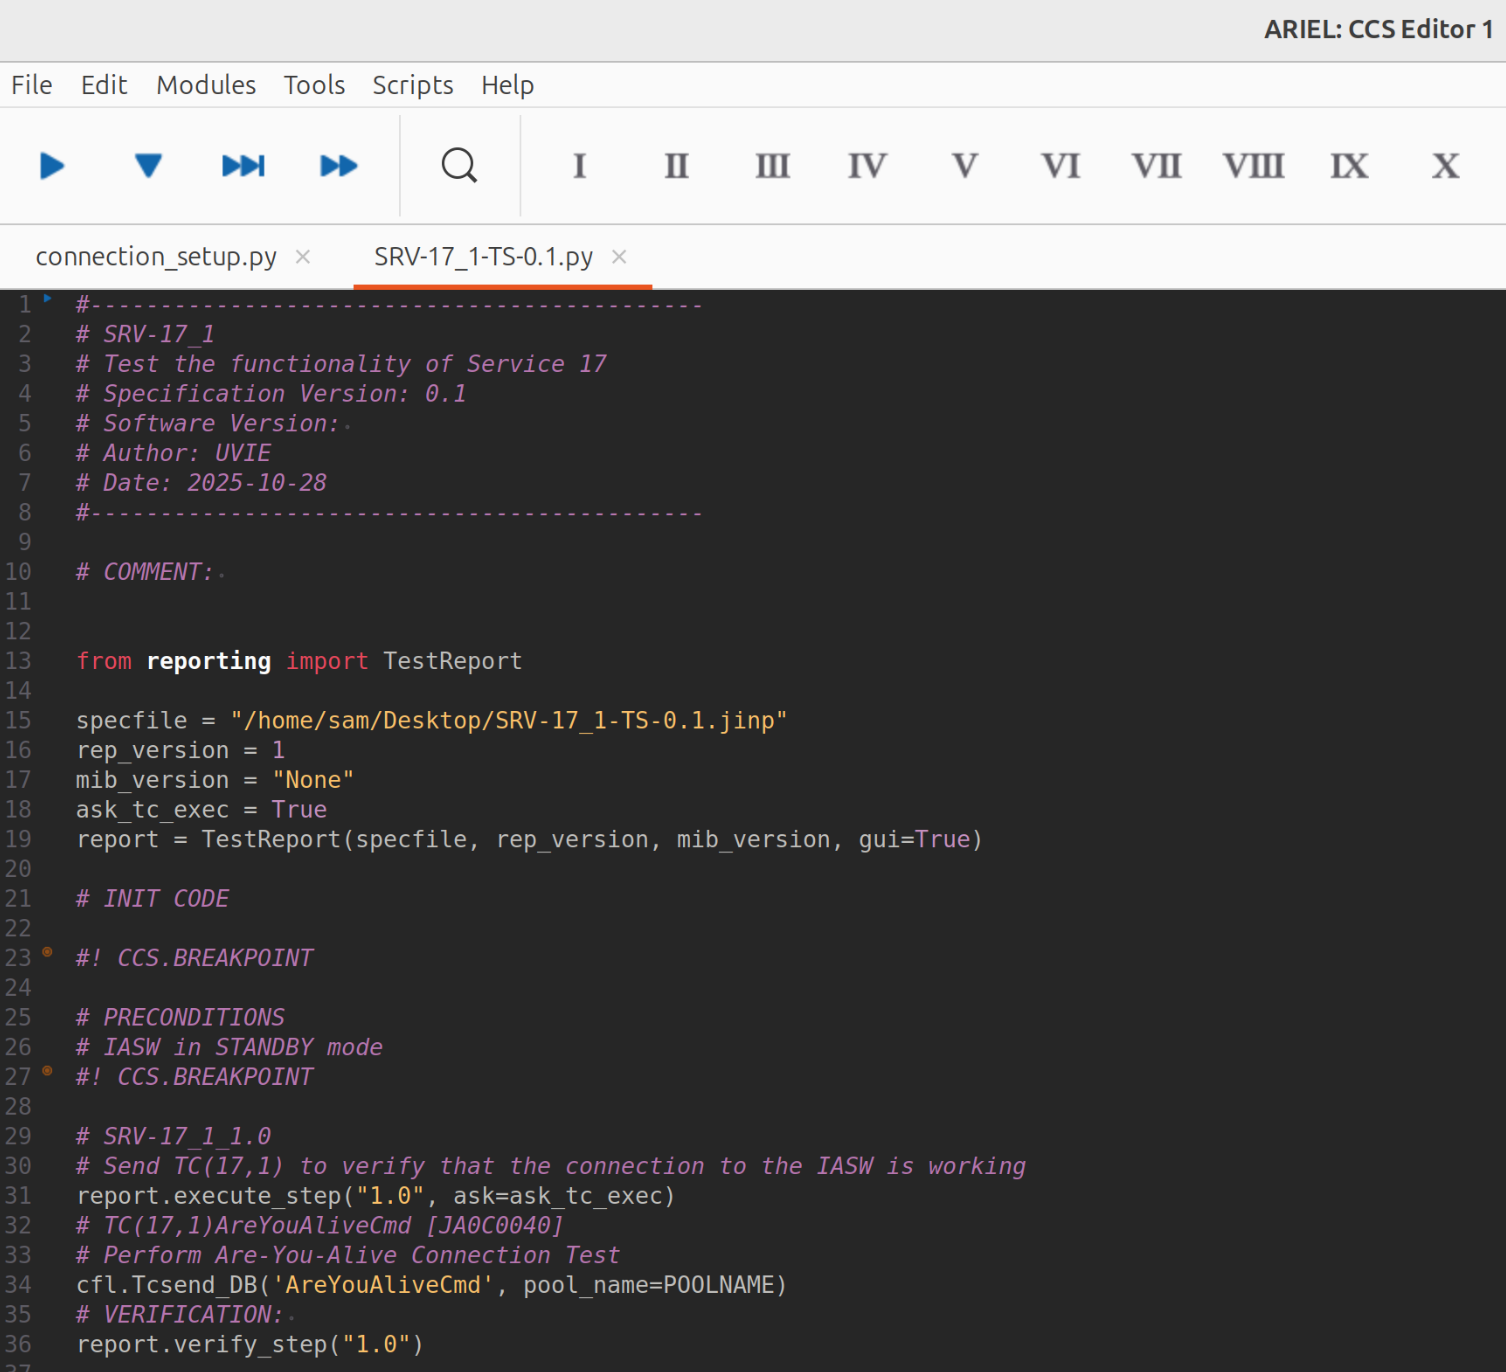
\includegraphics[width=0.8\linewidth]{test_editor.png}
    \caption{Generated test script displayed in \textit{ccs} editor}
    \label{fig:test_editor}
\end{figure}

\begin{figure}
    \centering
    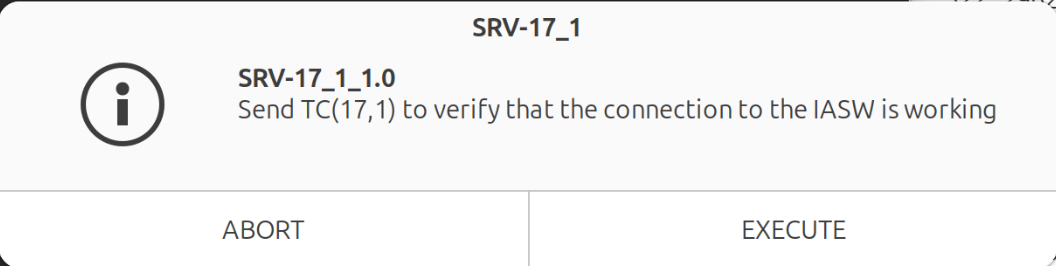
\includegraphics[width=0.5\linewidth]{dialog_1.png}
    \caption{Dialogue of a test script asking to execute a command}
    \label{fig:dialog_1}
\end{figure}


\begin{figure}
    \centering
    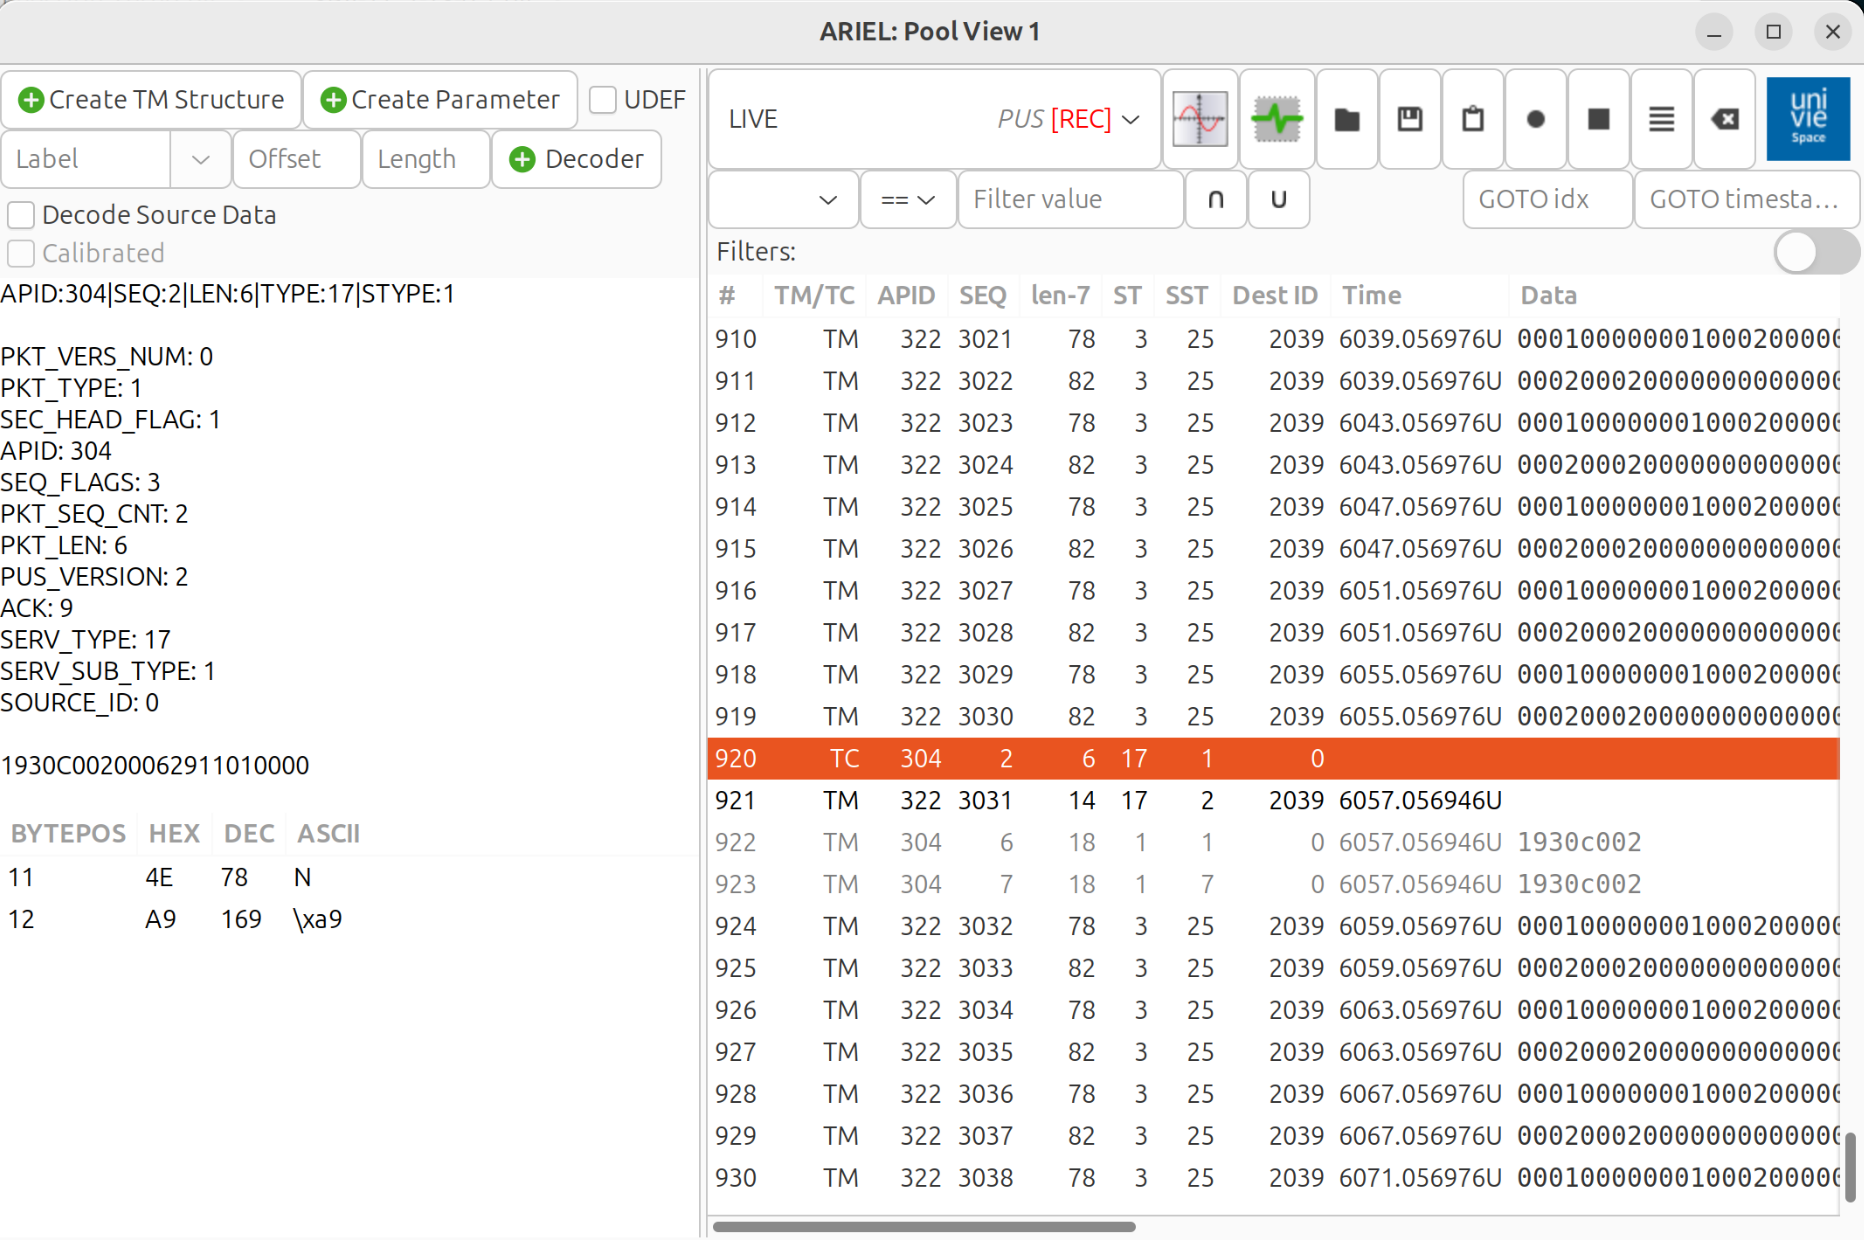
\includegraphics[width=0.8\linewidth]{test_viewer.png}
    \caption{Pool viewer displaying a command which was sent from the test script}
    \label{fig:test_viewer}
\end{figure}

A second dialogue then opens (Figure~\ref{fig:dialog_2}), allowing the user to document the result: 
The associated telemetry packets can be dragged and dropped into the telemetry table. 
Additional manual entries can be added using the “+” button and double clicking the empty line. 
Entries can be rearranged with the arrow buttons or deleted with the corresponding remove icon. 
The checkboxes determine which entries will appear in the final report. For commands with payload data, individual parameters may also be selected.

\begin{figure}
    \centering
    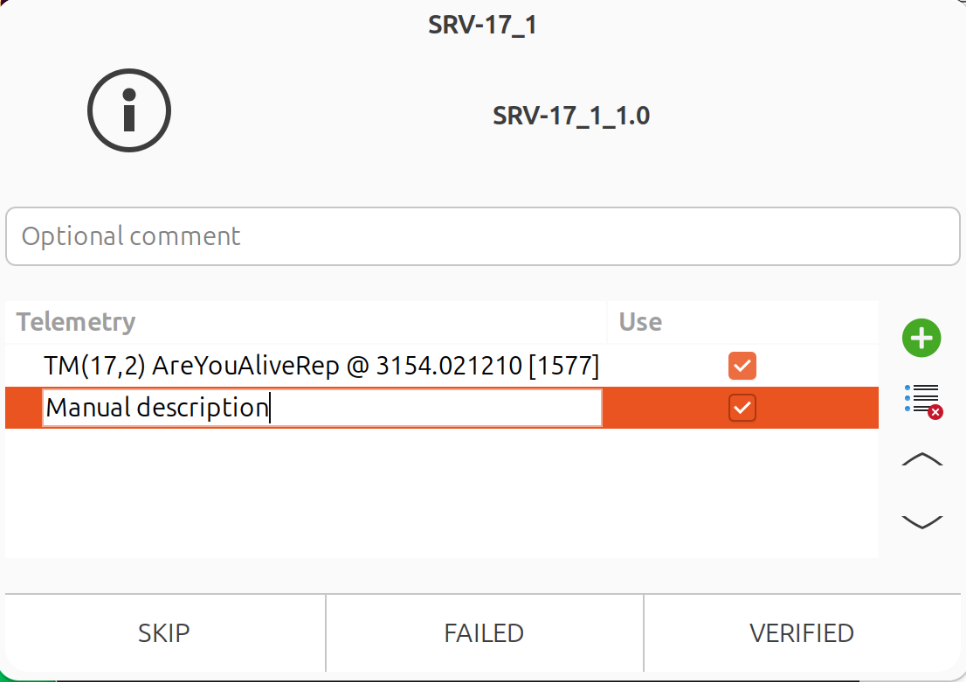
\includegraphics[width=0.5\linewidth]{dialog_2.png}
    \caption{Dialogue of a test script asking for comments and verification}
    \label{fig:dialog_2}
\end{figure}

At the bottom of the window, the following actions are available:

\begin{itemize}
    \item Skip: The step is omitted from the report
    \item Failed: Marks the step as failed in the report
    \item Verified: Confirms successful verification
\end{itemize}


Selecting “Verified” finalizes the step and proceeds to the next one, continuing the process until the test is complete. 
In the case of the example, a dialogue will appear asking "Wait for TM(17,2)" and a final verification window will show up. \\

If the Abort button is selected during any step, note that execution will stop at the current position. 
To restart the test from the beginning, the blue arrow icon in the \textit{ccs} editor must be reset to the top of the script.
Otherwise, clicking the Play button will resume execution from the next step. \\

Once the last step has been executed, an additional confirmation (a breakpoint) is encountered before the final report is generated. 
To produce the report, the user must execute the script one final time (i.e., press the blue arrow once more) after the last dialogue has closed. 
The generated report is saved automatically in the same directory as the test file, with the extension .jrep. 
This file contains all step outcomes, comments, and verification details recorded during the session.


%###########################################################################################
\chapter{Console commands} \label{scripts}
The \textit{ccs} editor integrates a full interactive IPython console, allowing users to execute Python commands, inspect functions, and interact directly with the connected system. 
This makes it an ideal environment for testing individual commands or for building and debugging scripts.

%###########################################################################################
\section{Documentation}
Within the console, users can enter any valid Python or \textit{ccs} command.
To quickly inspect a function, IPython provides two highly useful introspection tools:

\begin{itemize}
    \item ?: displays the docstring of a function
    \item ??: displays the source code of the function
\end{itemize}

To exit the documentation or source view, simply press the q key. 
This feature is particularly useful for quickly reviewing \textit{ccs} library functions such as Tcsend\_DB or Tcbuild, without having to open their corresponding source files manually. \\
For example when typing \texttt{Tcsend\_DB?} the Signature and Docstring are displayed and further explainations are given below as this is an essential command. 

\begin{figure}
    \centering
    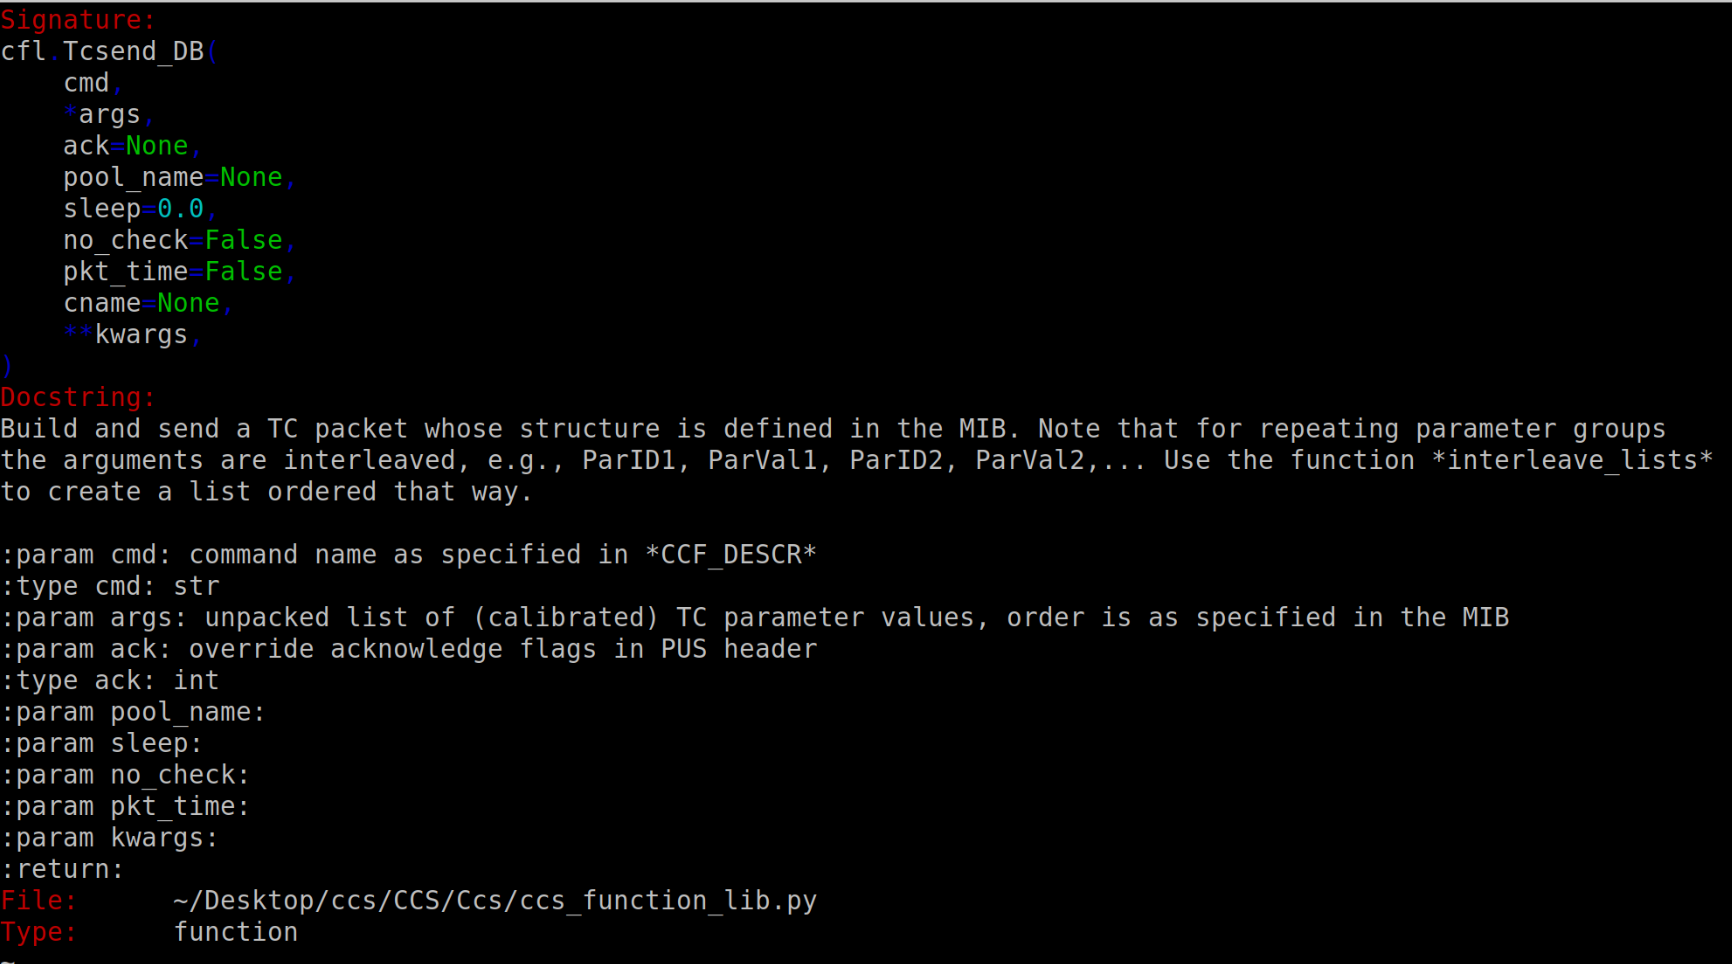
\includegraphics[width=0.5\linewidth]{Tcsend_DB?.png}
    \caption{Documentation for the command Tcsend\_DB}
    \label{fig:tcsend}
\end{figure}

\begin{itemize}
    \item cmd: command name exactly as defined in the mib

    \item args: list of arguments for commands with repeating parameters

    \item ack: acknowledgment flag in the PUS header - which service 1 TM packets are expected in response, for example ack=0b1011 will give TM(1,1), TM(1,3) and TM(1,7)

    \item pool\_name: data pool name through which the packet is sent, for example 'LIVE'

    \item sleep: pauses execution after sending a TC, for example, sleep=1.0 blocks subsequent commands for one second

    \item no\_check: normally, \textit{ccs} checks whether parameter values are valid before sending, setting no\_check = True \textit{ccs} to send the packet even if parameters are invalid (alternatively, use Tcbuild(), modify the packet and send it using Tcsend())

    \item pkt\_time: add a time reference to the TC based on the timestamp of the last TM packet in the pool

    \item cname: internal short name, from mib, used to resolve ambiguous or overly long command names (usually not required unless the command name is duplicated) 
\end{itemize}


%###########################################################################################
\section{Ccs Function Library}
The \texttt{cfl} module (short for \textit{ccs} function library) is a collection of useful functions which are also used internally by the \textit{ccs} system.
It is the main library for common tasks such as sending and receiving packets, handling telemetry, and interacting with the connected instruments.

Functions include, for example: \texttt{cfl.Tcsend\_DB()} – sends a TC packet defined in the MIB or \texttt{cfl.Tcbuild()} – builds a TC packet without sending it immediately.
These functions allow users to execute \textit{ccs} operations directly from the console or from within a Python script executed in the editor. 
An overview of useful functions is given in Sec.~\ref{functions}.
%A command which sends a TC to the application, will return the APID, Sequence count and internal time stamp of the sent TC as confirmation.
%A command can directly be dragged and dropped from the test tool into the upper section of the \textit{ccs} editor.\\

%###########################################################################################
\subsection{Control modules via editor}
Sometimes, one of the \textit{ccs} modules may not operate correctly. In such cases, it can manually be started directly from the editor console using cfl with optional debugging options. 
For instance the command \texttt{cfl.start\_pv(console=True)} launches the Pool Viewer and opens its console output inside the \textit{ccs} editor terminal.
Setting the option console=True is especially useful for debugging, since one can directly see error messages or log output.
Note: One can also check active communication links by entering \texttt{cfl.communication}, which lists all currently connected \textit{ccs} modules and their communication status. 
A value of 1 means the link is active.

%###########################################################################################
\subsection{Command with repeating parameters}
Some TCs include repeating parameter groups. This means that one or more parameters (like SID and period) can appear multiple times within the same packet. 
An example of such a command is TC(3,31) – ModHkPeriodCmd. 

If only one parameter group is used, the command is sent in a straightforward way:

\begin{verbatim}
NParam = 1 
SidNoCal = 2 
Period = 60 

cfl.Tcsend_DB('ModHkPeriodCmd', NParam, SidNoCal, Period, pool_name=POOLNAME)

\end{verbatim}


If more than one parameter group is required, a tuple cannot simply be passed. 
Instead, \textit{ccs} expects a flat, ordered list of interleaved parameters like (SID\_1, Period\_1,..., SID\_n, Period\_n). 
To build this list correctly, \textit{ccs} provides a function called \texttt{cfl.interleave\_lists()}, which takes multiple lists or tuples and interleaves their elements in the correct order.

Example for two parameter groups:
\begin{verbatim}
NParam = 2
SidNoCal = (1, 2)
Period = (40, 60)

cfl.Tcsend_DB('ModHkPeriodCmd', 
NParam, 
*cfl.interleave_lists(SidNoCal, Period), 
pool_name=POOLNAME)

\end{verbatim}

Note: The asterisk (*) in front unpacks the list so that each value is passed as an individual argument to Tcsend\_DB.



%###########################################################################################
\subsection{Send an illegal TC}
When wanting to test the applications reaction to faulty TCs, using Tcsend\_DB would be rather unhelpful. Instead, building the packet manually and sending the raw bytes using \texttt{Tcsend\_bytes()} allows for better manipulation. \\


\textbf{Using Tcbuild}\\
This method works by building a normal TC via the MIB and then manually breaking the bytes.

\begin{verbatim}
# Build a correct TC via the MIB
tc, (st, sst, apid) = cfl.Tcbuild('SASW AreYouAliveCmd')

# Corrupt the packet length (byte 5) and remove the crc completely
tc = tc[:5] + b'\x07' + tc[6:-2]

# Recalculate crc for the manipulated packet
crc = cfl.crc(tc).to_bytes(2, 'big')

# Append the new crc
tc = tc + crc

# Send the modified TC as raw bytes
cfl.Tcsend_bytes(tc, pool_name='LIVE')

\end{verbatim}

\textbf{Using Tcpack} \\
Tcpack creates a PUS TC directly at the byte level so the MIB is obsolete.

\begin{verbatim}
# Create some dummy payload
payload = b'\x01\x02\x03\x04'

# Build a PUS TC for a non-existent service 999
tc = cfl.Tcpack(
    data=payload,
    apid=304,
    st=999,
    sst=1,
    sdid=0,
    ack=0b0000)

# Send the illegal TC as raw bytes
cfl.Tcsend_bytes(tc, pool_name='LIVE')

\end{verbatim}



%###########################################################################################
\subsection{Extracting a packet}
This section describes the full workflow for retrieving packets from a \textit{ccs} data pool, selecting the desired ones and decoding them into readable information.
The process consists of three main stages: Query packets from the SQL database, filter the packets, decode the packets. 

Every pool stored in the database can be accessed using:\\
\texttt{rows = cfl.get\_pool\_rows("LIVE")}

This will return a SQLAlchemy query object (essentially a database reference), which still needs to be queried to yield actual rows. 
The rows query object, can be filtered by: service type, subservice type, apid, sid, etc. using: \\
\texttt{y = cfl.filter\_rows(rows, st=3, sst=25)}

As y is still a query object, certain operations are allowed like the following.

\begin{itemize}
    \item y.first(): first matching packet row
    \item y.all(): list of all matching rows (iteration possible)
    \item y.all()[-1]: last packet
    \item y.all()[-2]: second last, etc.
\end{itemize}

Each row contains the actual TM packet as a bytestring, accessible via:\\
\texttt{tm\_bytes = q.raw}\\

q.raw returns the bytestring of one packet, if several packets should be decoded, simply iterate over the rows:\\
\begin{verbatim}
for row in y.all():
    tm_bytes = row.raw
    ...
\end{verbatim}

This is the binary PUS TM packet. From here on, many operations can be done with the raw packet like converting to cuc time, computing the crc, inspecting the header, etc. (See Section \ref{functions})

\texttt{cfl.Tmread(tm\_bytes)} will return decoded header fields, raw data field, crc bytes \\
\texttt{cfl.Tmdata(tm\_bytes)} will return the name of the TM packet (based on MIB) and a list of parameter values\\
\texttt{print(cfl.Tmformatted(tm\_bytes))} will return a human-readable, formatted list of parameters \\
\texttt{cuc\_string = cfl.mkcucstring(tm\_bytes)} will return the seconds.microseconds timestamp including the U/S flag \\
\texttt{crc\_result = cfl.crc(tm\_bytes)} will compute the crc. If crc\_result == 0: crc matches, packet is valid. If crc\_result != 0: CRC fails, packet is corrupted.



%###########################################################################################
\subsection{Commonly used cfl functions} \label{functions}
The \textit{ccs} Function Library provides a large set of helper routines that allows the user to interact with the \textit{ccs} subsystems directly from the console or within scripts.
While not all of them are required for everyday testing, a number of key functions are used frequently for sending telecommands, handling telemetry, and managing the communication between modules.\\


%###########################################################################################

\begin{table}[h!]
\centering
\renewcommand{\arraystretch}{1.3}
\setlength{\tabcolsep}{8pt}
\begin{tabular}{p{4cm} p{5cm} p{6cm}}
\hline
\textbf{Function} & \textbf{Arguments} & \textbf{Description} \\ 
\hline


\texttt{cfl.start\_pv} & \texttt{pool\_name=None, console=False, **kwargs} & Launches the Pool Viewer for the given pool. With \texttt{console=True}, routes module output to the Editor console for debugging (same functionality for all following functions). \\

\texttt{cfl.start\_pmgr} & \texttt{gui=True, console=False, **kwargs} & Launches the Pool Manager, set \texttt{gui=False} to run without a window. \\

\texttt{cfl.start\_editor} & \texttt{*files, console=False, **kwargs} & Launches the Editor, optional \texttt{*files} are opened as tabs.\\

\texttt{cfl.start\_monitor} & \texttt{pool\_name, parameter\_set=None, console=False, **kwargs} & Launches the Parameter Monitor for the given pool. Optionally preselect a \texttt{parameter\_set}. \\

\texttt{cfl.start\_plotter} & \texttt{pool\_name, console=False, **kwargs} & Launches the Parameter Plotter for the given pool. \\

\texttt{cfl.start\_config\_editor} & \texttt{console=False, **kwargs} & Launches the Configuration Editor for viewing and modifying \texttt{.cfg} files. \\

\texttt{cfl.start\_tst} & \texttt{console=False, **kwargs} & Opens the Test Specification Tool for defining and executing test sequences.\\

\texttt{cfl.connect} & \texttt{pool\_name, host, port, protocol='PUS', is\_server=False, timeout=10, delete\_abandoned=False, try\_delete=True, pckt\_filter=None, options='', drop\_rx=False, drop\_tx=False} & Establishes a general connection between \textit{ccs} and a target (e.g. simulation or instrument). Creates a link for streams via the Pool Manager. Handles socket creation and optional filtering. \\

\texttt{cfl.connect\_tc} & \texttt{pool\_name, host, port, protocol='PUS', drop\_rx=True, timeout=10, is\_server=False, use\_socket=None, options=''} & Specifically establishes a TC channel to the target. Usually called after \texttt{connect()} for systems that separate TM and TC communication ports. \\


\hline
\end{tabular}
\caption{Commonly used CCS Function Library (cfl) commands for module control.}
\end{table}


\begin{table}[h!]
\centering
\renewcommand{\arraystretch}{1.3}
\setlength{\tabcolsep}{8pt}
\begin{tabular}{p{4cm} p{5cm} p{6cm}}
\hline
\textbf{Function} & \textbf{Arguments} & \textbf{Description} \\ 
\hline

\texttt{cfl.mkcucstring} & \texttt{tml} & Generates a CUC time string (format: \texttt{seconds.microseconds U/S}) from a telemetry packet or decoded TM header (binary arguments). Time is synchronized: (\texttt{S}) or unsynchronized (\texttt{U}). \\

\texttt{cfl.get\_cuc\_now} & - & Returns the current time in seconds since the CUC reference epoch. \\

\texttt{cfl.utc\_to\_cuc} & \texttt{utc} & Converts a UTC timestamp (ISO string or timezone-aware datetime) into seconds since the CUC reference epoch. \\

\texttt{cfl.cuc\_to\_utc} & \texttt{cuc} & Converts CUC time (seconds since reference epoch) into an ISO-formatted UTC string. \\

\texttt{cfl.cuc\_to\_date} & \texttt{cuc} & Converts CUC time to a datetime object. \\
\hline
\end{tabular}
\caption{Commonly used CCS Function Library (cfl) commands for time management.}
\end{table}




%###########################################################################################


\begin{table}[h!]
\centering
\renewcommand{\arraystretch}{1.3}
\setlength{\tabcolsep}{8pt}
\begin{tabular}{p{4cm} p{5cm} p{6cm}}
\hline
\textbf{Function} & \textbf{Arguments} & \textbf{Description} \\ 
\hline

\texttt{cfl.collect\_13} & \texttt{pool\_name, starttime=None, endtime=None, startidx=None, endidx=None, join=True, collect\_all=False, sdu=None, verbose=True, consistency\_check=True} &
Collects and groups PUS Service 13 downlinks trains from a pool (or from DB if \texttt{pool\_name} is not a file).  
Supports time/index windows and optional SDU selector.  
If \texttt{collect\_all=False} only the first complete transfer is returned; with \texttt{join=True} segments are concatenated.  
Returns a dict where each value timestamp is the key for the transferred data. \\

\texttt{cfl.dump\_large\_data} & \texttt{pool\_name, starttime=0, endtime=None, outdir="", dump\_all=False, sdu=None, startidx=None, endidx=None, verbose=True, consistency\_check=True} &
Dumps Service 13 downlink data to disk. Internally uses \texttt{collect\_13}. 
For pools loaded from a file, pool\_name must be the absolute path of that file. \\

\texttt{cfl.load\_to\_memory} & \texttt{data, memid, memaddr, max\_pkt\_size=MAX\_PKT\_LEN, sleep=0.125, ack=0b1001, pool\_name='LIVE', tcname=None, progress=True, calc\_crc=True, byte\_align=4, dryrun=False} &
Uploads a byte buffer (or file path) into target memory at \texttt{memaddr} for the given \texttt{memid}.  
Splits into TC(6,2) packets, ensures payload alignment.  
\emph{Returns} \texttt{(total\_bytes, crc)} over the uploaded data if \texttt{calc\_crc=True}; otherwise \texttt{None}. With \texttt{dryrun=True} no packets are sent. \\

\texttt{cfl.upload\_srec} & \texttt{fname, memid, pool\_name='LIVE', max\_pkt\_size=MAX\_PKT\_LEN, tcname=None, sleep=0.125, progress=True, image\_crc=True, byte\_align=2, ack=0b1001, dryrun=False} &
Uploads an Intel/Motorola S-record image directly to memory \texttt{memid}, optional image crc.  
\emph{Returns} whatever \texttt{srec\_direct} returns, or \texttt{None} in dry-run. \\


\hline
\end{tabular}
\caption{Commonly used CCS Function Library (cfl) commands for data acquisition and handling as well as moving large binaries betweem host and target memory.}
\end{table}



%###########################################################################################

\begin{table}[h!]
\centering
\renewcommand{\arraystretch}{1.3}
\setlength{\tabcolsep}{8pt}
\begin{tabular}{p{4cm} p{5cm} p{6cm}}
\hline
\textbf{Function} & \textbf{Arguments} & \textbf{Description} \\ 
\hline

\texttt{cfl.get\_pool\_rows} & \texttt{pool\_name, check\_existence=False} &
Returns a SQL query object containing all telemetry rows belonging to the given pool.  
If \texttt{check\_existence=True}, it will raise an error when the pool does not exist.  
Useful as a base query for further manipulation. \\


\texttt{cfl.get\_data\_pool\_items} & \texttt{pcf\_descr=None, src\_file=None, as\_dict=False} &
Loads data-pool parameter definitions either directly from a plain-text file (\texttt{src\_file}), or from the PCF table.  
Can return a list of tuples or a dictionary keyed by PID (\texttt{as\_dict=True}). \\

\texttt{cfl.extract\_pus} & \texttt{data} & 
Extracts all PUS packets from a byte buffer or file-like object.  
\emph{Returns} a list of decoded PUS packets.  \\

\texttt{cfl.filter\_rows} & \texttt{rows, st=None, sst=None, apid=None, sid=None, time\_from=None, time\_to=None, idx\_from=None, idx\_to=None, tmtc=None, get\_last=False, sid\_lu\_apid=None} &
Function to filter a pool row-query by any combination of  
ST, SST, APID, SID, timestamps, index ranges, or TM/TC type.  
With \texttt{get\_last=True} it returns the most recent matching entry.  
\emph{Returns} a filtered SQLAlchemy query (or a single row when \texttt{get\_last}). \\

\hline
\end{tabular}
\caption{Commonly used CCS Function Library (cfl) commands for data pool handling: filtering and extraction of PUS fields or decoded items from the current data pool.}
\end{table}




%###########################################################################################

\begin{table}[h!]
\centering
\renewcommand{\arraystretch}{1.3}
\setlength{\tabcolsep}{8pt}
\begin{tabular}{p{4cm} p{5cm} p{6cm}}
\hline
\textbf{Function} & \textbf{Arguments} & \textbf{Description} \\ 
\hline

\texttt{cfl.savepool} & \texttt{filename, pool\_name, mode='binary', st\_filter=None} &
Saves the full content of a data pool to disk.  
The file can be written either as raw binary (\texttt{mode='binary'}) or as a human-readable hex dump.  
\texttt{st\_filter} allows exporting only packets of a specific service type.  \\

\texttt{DbTools.recover\_from\_db} & \texttt{pool\_name=None, iid=None, dump=False} &
Recovers TM/TC packets that remain only in the database (not saved to disk).  
Identify the pool either by \texttt{pool\_name} or by its internal ID \texttt{iid}.  
If \texttt{dump} is a filename, all recovered raw packets are written directly to that file.  
Must be used before a new pool is started! \\

\texttt{DbTools.clear\_from\_db} & \texttt{pool\_name, answer=''} &
Deletes a single pool (and all its packets) from the database. \\

\texttt{DbTools.\_clear\_db} & \texttt{-} &
Deletes \emph{all} TM/TC pools and all TM packets from the database.  
This completely resets the CCS telemetry database. This can also be achived by using the \texttt{make database} command in the terminal which was first used for installation. \\

\texttt{DbTools.\_purge\_db\_logs} & \texttt{date=None} &
Purges MySQL binary logs older than the given timestamp.  
If \texttt{date=None}, the current date/time is used. \\
\hline

\hline
\end{tabular}
\caption{Commonly used CCS Function Library (cfl) commands for data pool management:  persist pools to disk, rebuild them from the database or clear old data.}
\end{table}


%###########################################################################################

\begin{table}[h!]
\centering
\renewcommand{\arraystretch}{1.3}
\setlength{\tabcolsep}{8pt}
\begin{tabular}{p{4cm} p{5cm} p{6cm}}
\hline
\textbf{Function} & \textbf{Arguments} & \textbf{Description} \\ 
\hline

\texttt{cfl.Tcdata} & \texttt{tm} &
Decodes a TC packet (given as raw bytes or DB row) using the MIB.  
Internally determines ST/SST/APID, resolves discriminants, and extracts all TC parameters with their calibrated values.  
Returns: a list of decoded parameters or \texttt{None} \\

\texttt{cfl.Tcsend\_DB} & \texttt{cmd, *args, ack=None, pool\_name=None, sleep=0., no\_check=False, pkt\_time=False, cname=None, mib\_head=False} &
Builds and sends a telecommand based on its MIB definition.  
Handles parameter packing, ACK flags, sequence counters, and sending via the PoolManager.  
\texttt{no\_check=True} forces \textit{ccs} to send even invalid parameters.  
Returns \texttt{True/False} depending on send success. \\

\texttt{cfl.Tcbuild} & \texttt{cmd, *args, sdid=0, ack=None, no\_check=False, hack\_value=None, source\_data\_only=False, fmt='raw', cname=None, mib\_head=False} &
Builds a TC byte-string from its MIB entry without sending it.  
Supports: variable-length TCs, test values, returning only source data
Returns either a PUS packet (as bytes), or MIB header information. \\

\texttt{cfl.Tcpack} & \texttt{data=b'', apid=0x14c, st=1, sst=1, sdid=0, version=0, typ=1, dhead=1, gflags=0b11, sc=None, tmv=PUS\_VERSION, ack=0b1001, pktl=None, chksm=None, **kwargs} &
Low-level creator of a PUS-compliant TC packet.  
Constructs full CCSDS + PUS headers, sets sequence counters, inserts crc.  
Returns the raw TC packet bytes. \\

\texttt{cfl.Tcsend\_bytes} & \texttt{tc\_bytes, pool\_name='LIVE', pmgr\_handle=None} &
Sends a fully constructed TC byte array directly to the PoolManager.  
Useful when manually constructing packets (e.g.\ from \texttt{Tcpack}).  
Returns \texttt{True} on success, \texttt{False} otherwise. \\

\texttt{cfl.get\_tc\_list} & \texttt{ccf\_descr=None, ccf\_cname=None} &
Queries the MIB for telecommand definitions.  
If \texttt{ccf\_cname} is given, only that command is returned,  
if \texttt{ccf\_descr} is given, it filters by the descriptive name,  
with both omitted, the full TC catalogue is returned.  
\emph{Returns} a dictionary keyed by TC identifiers with lists of parameter data. \\


\hline
\end{tabular}
\caption{Commonly used CCS Function Library (cfl) commands for handling, manipulation and sendig of telecommands.}
\end{table}


%###########################################################################################

\begin{table}[h!]
\centering
\renewcommand{\arraystretch}{1.3}
\setlength{\tabcolsep}{8pt}
\begin{tabular}{p{4cm} p{5cm} p{6cm}}
\hline
\textbf{Function} & \textbf{Arguments} & \textbf{Description} \\ 
\hline


\texttt{cfl.Tmformatted} & \texttt{tm, separator="n", sort\_by\_name=False, textmode=True, udef=False, nocal=False, floatfmt=None} &
High level function that produces a readable text representation of a TM packet.  
Internally calls \texttt{Tmdata} to decode the source data.  
Options allow sorting by parameter name, disabling calibration, or returning table-like output.  
\emph{Returns} either a formatted string or a list/table structure (if \texttt{textmode=False}). \\

\texttt{cfl.Tmdata} & \texttt{tm, udef=False, floatfmt=None} &
Decodes the source data field of a TM packet according to MIB definitions.  
Extracts service type, subtype, APID, SPID, and parameter list, handles variable-length packets,  
and supports user-defined decoders (UDEF).  
\emph{Returns} a list of decoded parameter tuples and the TM names. \\

\texttt{cfl.Tmread} & \texttt{pckt} &
Low-level parser for TM bytestrings.  
Uses the PUS header to determine whether the packet is TM or TC, extracts the header, data field, and crc. 
\emph{Returns} \texttt{(header\_fields, data\_bytes, crc)}. \\


\texttt{cfl.Tmdump} & \texttt{filename, tmlist, mode='hex', st\_filter=None, check\_crc=False} & 
Write a list or generator of TM packets to disk.  
Supports hex, binary, and text (human readable via \texttt{Tmformatted}).  
Optional \texttt{st\_filter} and \texttt{check\_crc} allow saving only selected or crc clean packets. 
Use savepool when dumping a whole pool; use Tmdump when dumping a packet list (even just one packet).\\


\texttt{cfl.Tm\_filter\_st} & \texttt{tmlist, st=None, sst=None, apid=None, sid=None, time\_from=None, time\_to=None} &
Filter for a list of TM packets.  
Can restrict by service type and sub type, APID, SID, and cuc time interval.  
Returns a new list containing only packets that match all given criteria. \\


\hline
\end{tabular}
\caption{Commonly used CCS Function Library (cfl) commands for handling, manipulation and reading of telemetry.}
\end{table}



\begin{table}[h!]
\centering
\renewcommand{\arraystretch}{1.3}
\setlength{\tabcolsep}{8pt}
\begin{tabular}{p{4cm} p{5cm} p{6cm}}
\hline
\textbf{Function} & \textbf{Arguments} & \textbf{Description} \\ 
\hline

\texttt{cfl.Tmpack} & \texttt{data=b'', apid=321, st=1, sst=1, destid=0, version=0, typ=0, timestamp=0, dhead=1, gflags=0b11, sc=None, tmv=PUS\_VERSION, tref\_stat=0, msg\_type\_cnt=0, pktl=None, chksm=None} &
Low level constructor for a TM packet conforming to PUS.  
Builds the full PUS header (including sequence count and length), appends the payload and crc and returns the complete TM bytestring.  \\

\texttt{cfl.create\_hk\_decoder} & \texttt{sid, *dp\_ids, apid=None} &
Create a user defined decoder for custom housekeeping TM(3,25) packets that are not described in the MIB.  
Takes the HK \texttt{SID} and one or more data pool IDs (\texttt{dp\_ids}), optionally a specific \texttt{APID}.  
Returns the decoder label that will be used when decoding packets. \\

\texttt{cfl.interleave\_lists} & \texttt{*args} &
Utility to interleave multiple iterables element by element.  
Commonly used for TCs with repeating parameter groups (e.g.\ SID and period):  
\texttt{interleave\_lists((1,2), (40,60))} → \texttt{[1, 40, 2, 60]}. \\

\hline
\end{tabular}
\caption{Commonly used CCS Function Library (cfl) commands for handling, manipulation and reading of telemetry and telecommands.}
\end{table}


\end{document}